\documentclass[11pt]{article}

\usepackage[margin=1in]{geometry}
\usepackage[T1]{fontenc}
\usepackage[utf8]{inputenc}
\usepackage{lmodern}
\usepackage{microtype}
\usepackage{amsmath,amssymb,mathtools}
\usepackage{hyperref}
\usepackage{graphicx}
\usepackage{subcaption}
\usepackage{float}
\hypersetup{hidelinks}

\title{Short note on kernel GD experiments on $S^1$}
\author{Shreyas Kalvankar}
\date{\today}

\begin{document}
\maketitle

\section*{Setup}

We work on the equally spaced grid
\[
	\phi_j = \frac{2\pi j}{n}, \qquad j=0,\dots,n-1,
\]
and use the cosine features
\[
	c_k(\phi_j) = \cos(k\phi_j), \qquad k=0,1,2,3,\dots.
\]

The target is a cosine mixture
\[
	y(\phi)
	=
	\sum_{k=0}^3 \alpha_k \cos(k\phi).
\]
In the baseline run,
\[
	y(\phi)
	=
	1 + 0.9\cos(\phi) + 0.5\cos(2\phi) + 0.35\cos(3\phi).
\]

We compare two equally spaced grid experiments:
\begin{itemize}
	\item \textbf{grid\_1024}: $n=1024$ training points,
	\item \textbf{grid\_4096}: $n=4096$ training points.
\end{itemize}

Kernel gradient descent is run with
\[
	f_{t+1} = f_t - \eta K (f_t-y),
	\qquad
	K_{ij}=\Theta(\phi_i-\phi_j),
\]
and residual
\[
	r_t := f_t-y.
\]

Because the kernel is translation-invariant and the grid is equally spaced, the Fourier modes decouple exactly. If
\[
	K c_k = \lambda_k^{\mathrm{emp}} c_k,
\]
then the residual coefficient along mode $k$ satisfies
\[
	r_k(t+1) = (1-\eta\lambda_k^{\mathrm{emp}})\,r_k(t),
\]
hence
\[
	r_k(t)=(1-\eta\lambda_k^{\mathrm{emp}})^t r_k(0).
\]

For zero initialization, $y_0=0$, so
\[
	r_k(0)=-\alpha_k,
	\qquad
	r_k(t)=-\alpha_k(1-\eta\lambda_k^{\mathrm{emp}})^t.
\]
Thus:
\begin{itemize}
	\item $\alpha_k$ determines the initial size of mode $k$,
	\item $\lambda_k^{\mathrm{emp}}$ determines the decay rate.
\end{itemize}

To compare rates across grids, we normalize mode amplitudes by their initial values:
\[
	\frac{|r_k(t)|}{|r_k(0)|} = |1-\eta\lambda_k^{\mathrm{emp}}|^t.
\]

\section*{Continuum vs empirical eigenvalues}

The continuum operator is
\[
	(Tf)(\phi)
	=
	\int_0^{2\pi}\Theta(\phi-\psi)f(\psi)\,\frac{d\psi}{2\pi},
\]
with Fourier eigenvalues $\lambda_k^{\mathrm{cont}}$.

The discrete experiment uses the raw Gram matrix $K$, so on an equally spaced grid
\[
	K \approx n\,T_{\mathrm{disc}},
\]
and therefore
\[
	\lambda_k^{\mathrm{emp}} \approx n\,\lambda_k^{\mathrm{cont}}.
\]
Hence, when comparing across grid sizes, we normalize the empirical eigenvalues by $n$.

\section*{Results: grid comparison}

\subsection*{Final prediction and residual decay}

\begin{figure}[H]
	\centering
	\begin{subfigure}[t]{0.48\textwidth}
		\centering
		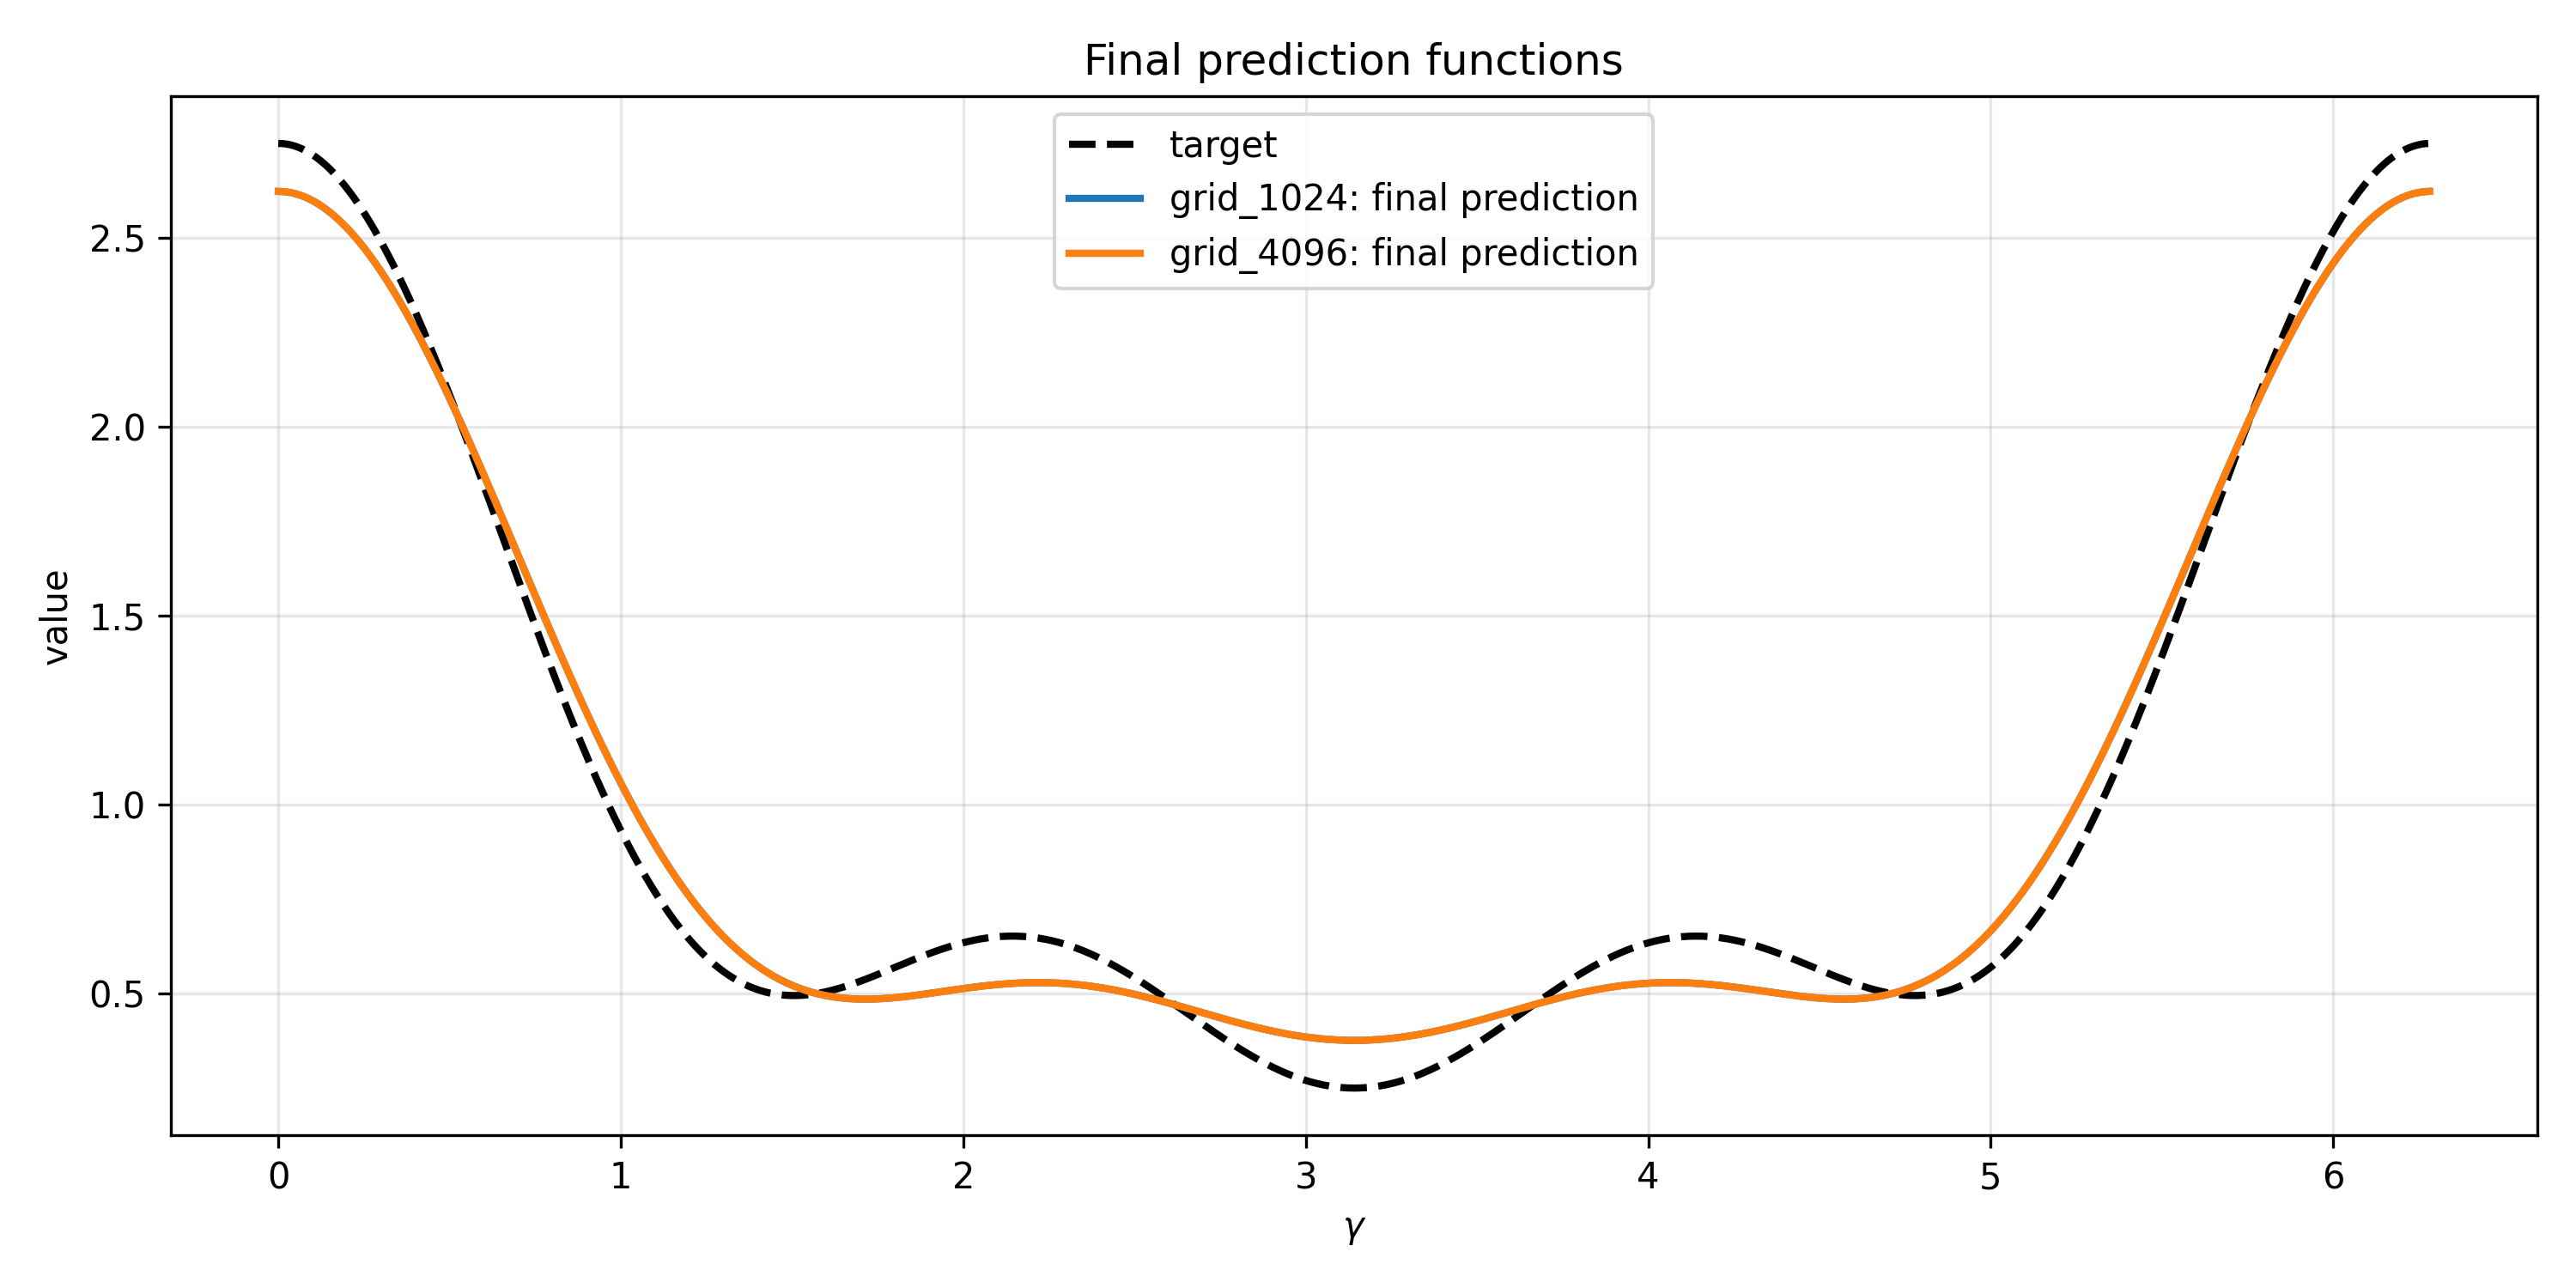
\includegraphics[width=\linewidth]{images/final_predictions_grid.png}
		\caption{Final prediction functions}
	\end{subfigure}
	\hfill
	\begin{subfigure}[t]{0.48\textwidth}
		\centering
		
\includegraphics[width=\linewidth]{images/loss_curve_grid.png}
		\caption{Loss / residual decay normalized by grid size}
	\end{subfigure}
	\caption{Comparison of the two grid experiments.}
\end{figure}

\paragraph{Observations.}
\begin{itemize}
	\item The final prediction curves for grid\_1024 and grid\_4096 are visually indistinguishable.
	\item Both runs converge to essentially the same fitted function after $1000$ steps.
	\item The normalized loss curves also overlap almost perfectly, indicating that the overall residual decay is the same at both grid resolutions.
	\item At this level, increasing the grid from $1024$ to $4096$ does not visibly improve the final fit.
\end{itemize}

\subsection*{Final prediction error}

\begin{figure}[H]
	\centering
	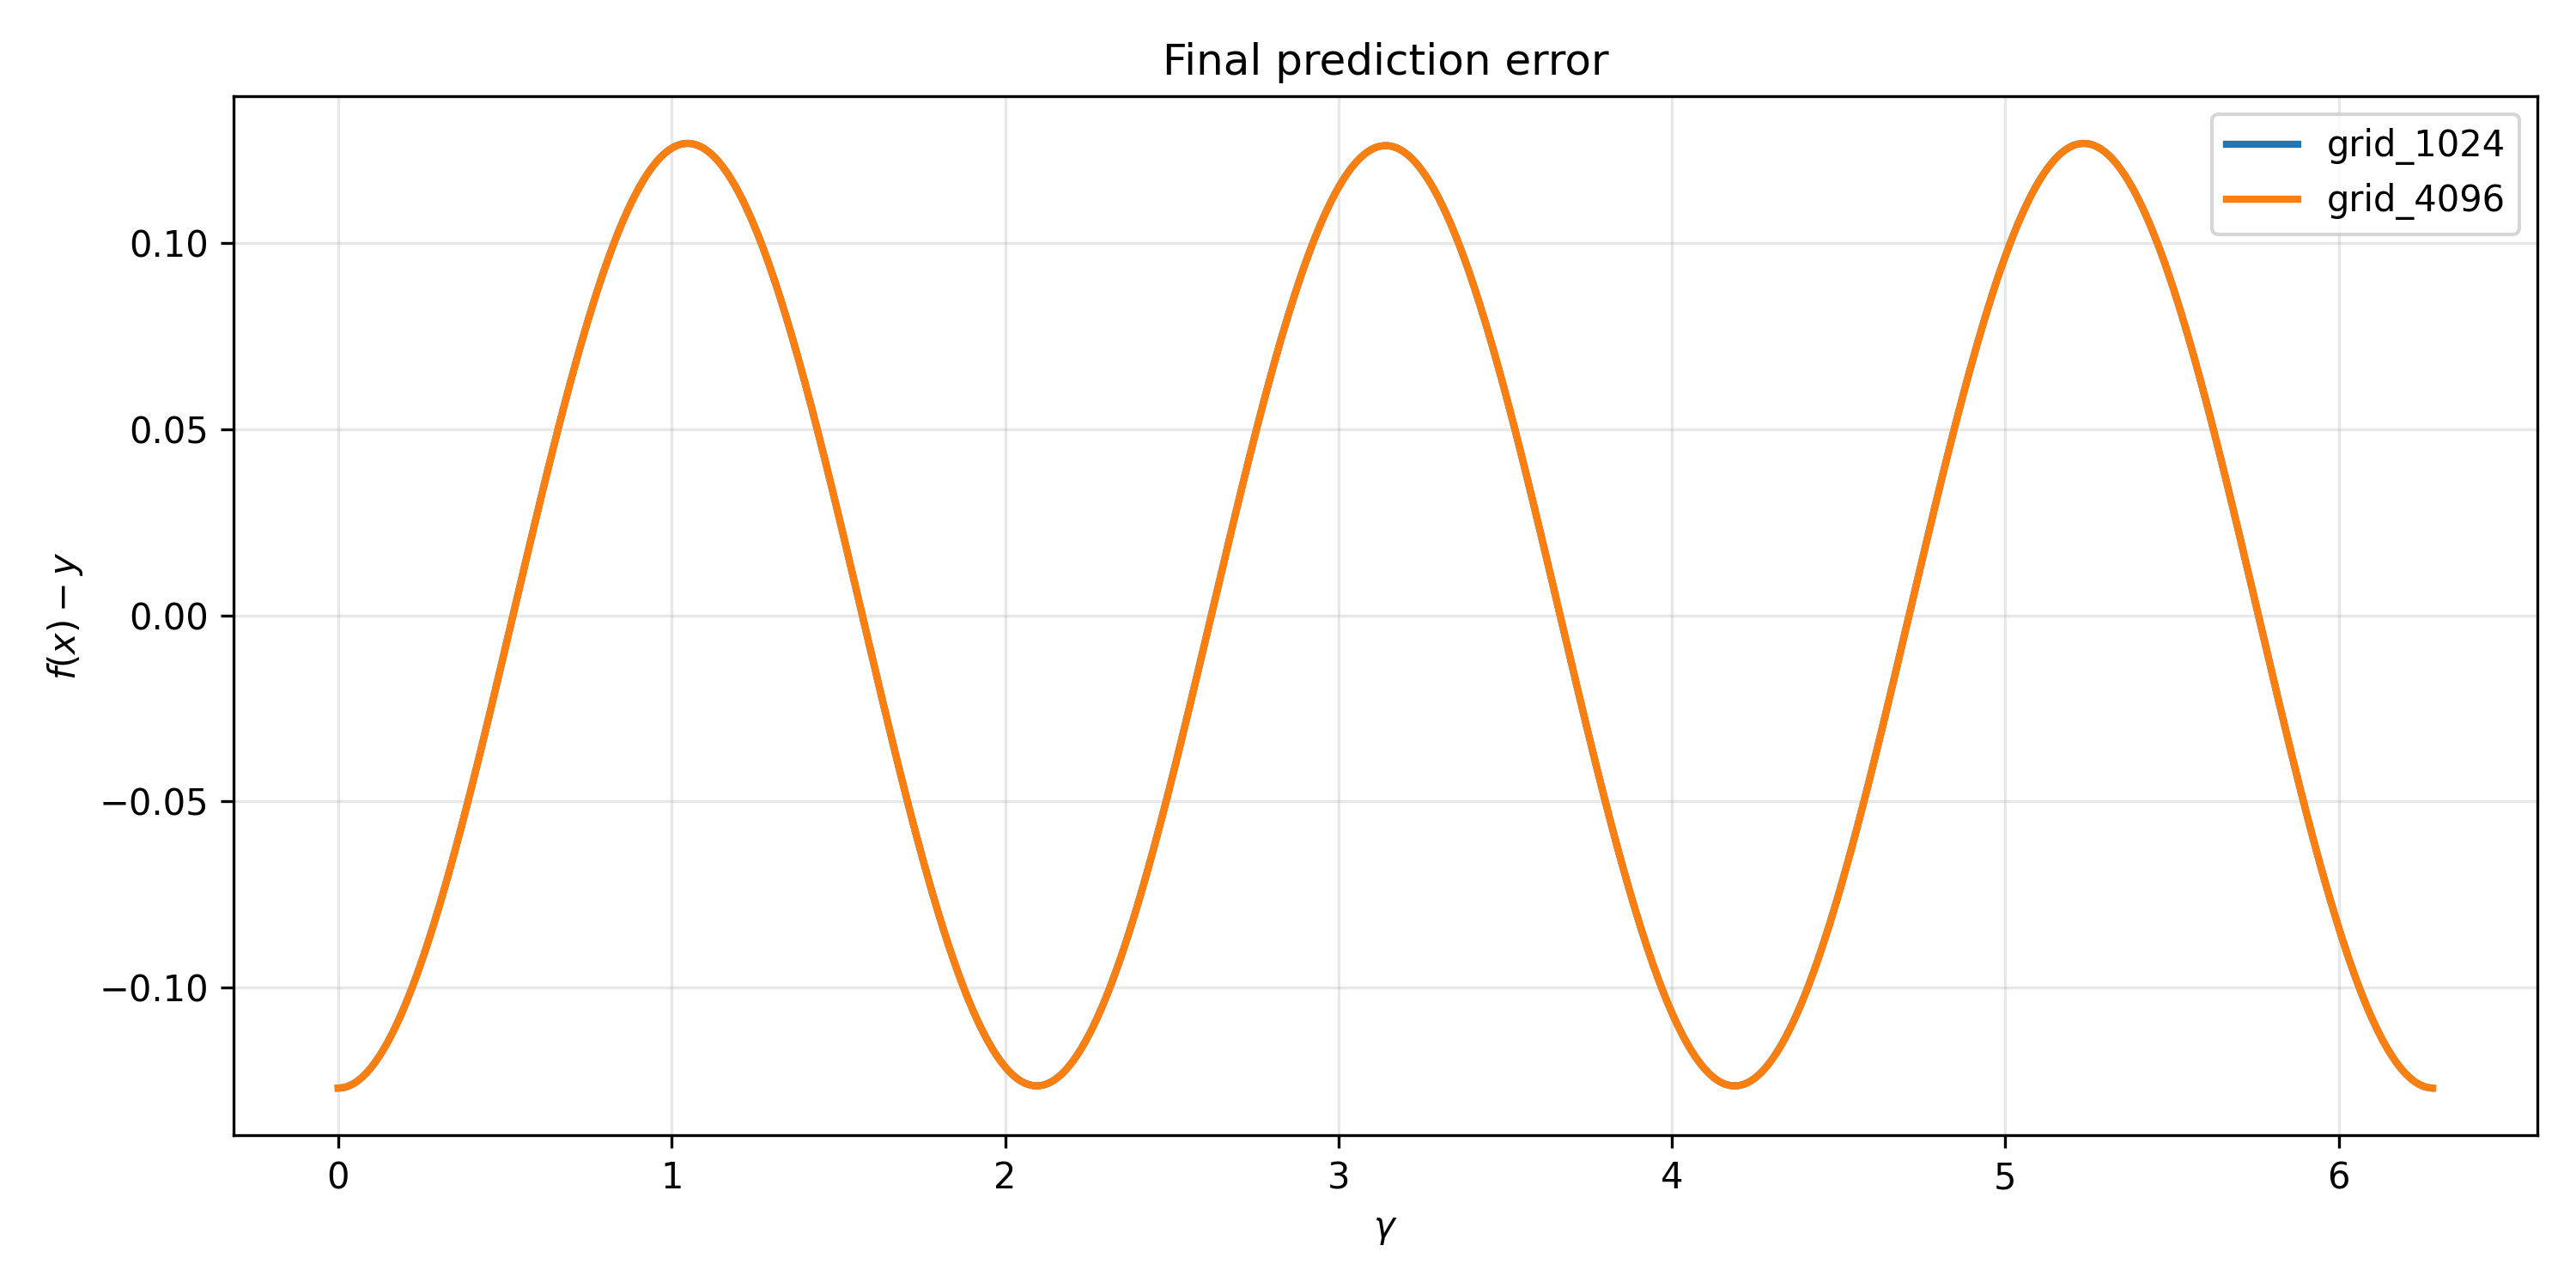
\includegraphics[width=0.68\textwidth]{images/prediction_error_grid.png}
	\caption{Final prediction error $f(x)-y$ for the two grid experiments.}
\end{figure}

\paragraph{Observations.}
\begin{itemize}
	\item The final error curves for grid\_1024 and grid\_4096 overlap almost exactly.
	\item The remaining error is exactly the high-frequency mode that wasn't learnt.
	\item This suggests that the residual error is not primarily due to coarse discretization at $n=1024$.
	\item Instead, the dominant effect here appears to be incomplete convergence of the slower modes within the chosen number of GD steps.
\end{itemize}

\subsection*{Spectrum comparison}

\begin{figure}[H]
	\centering
	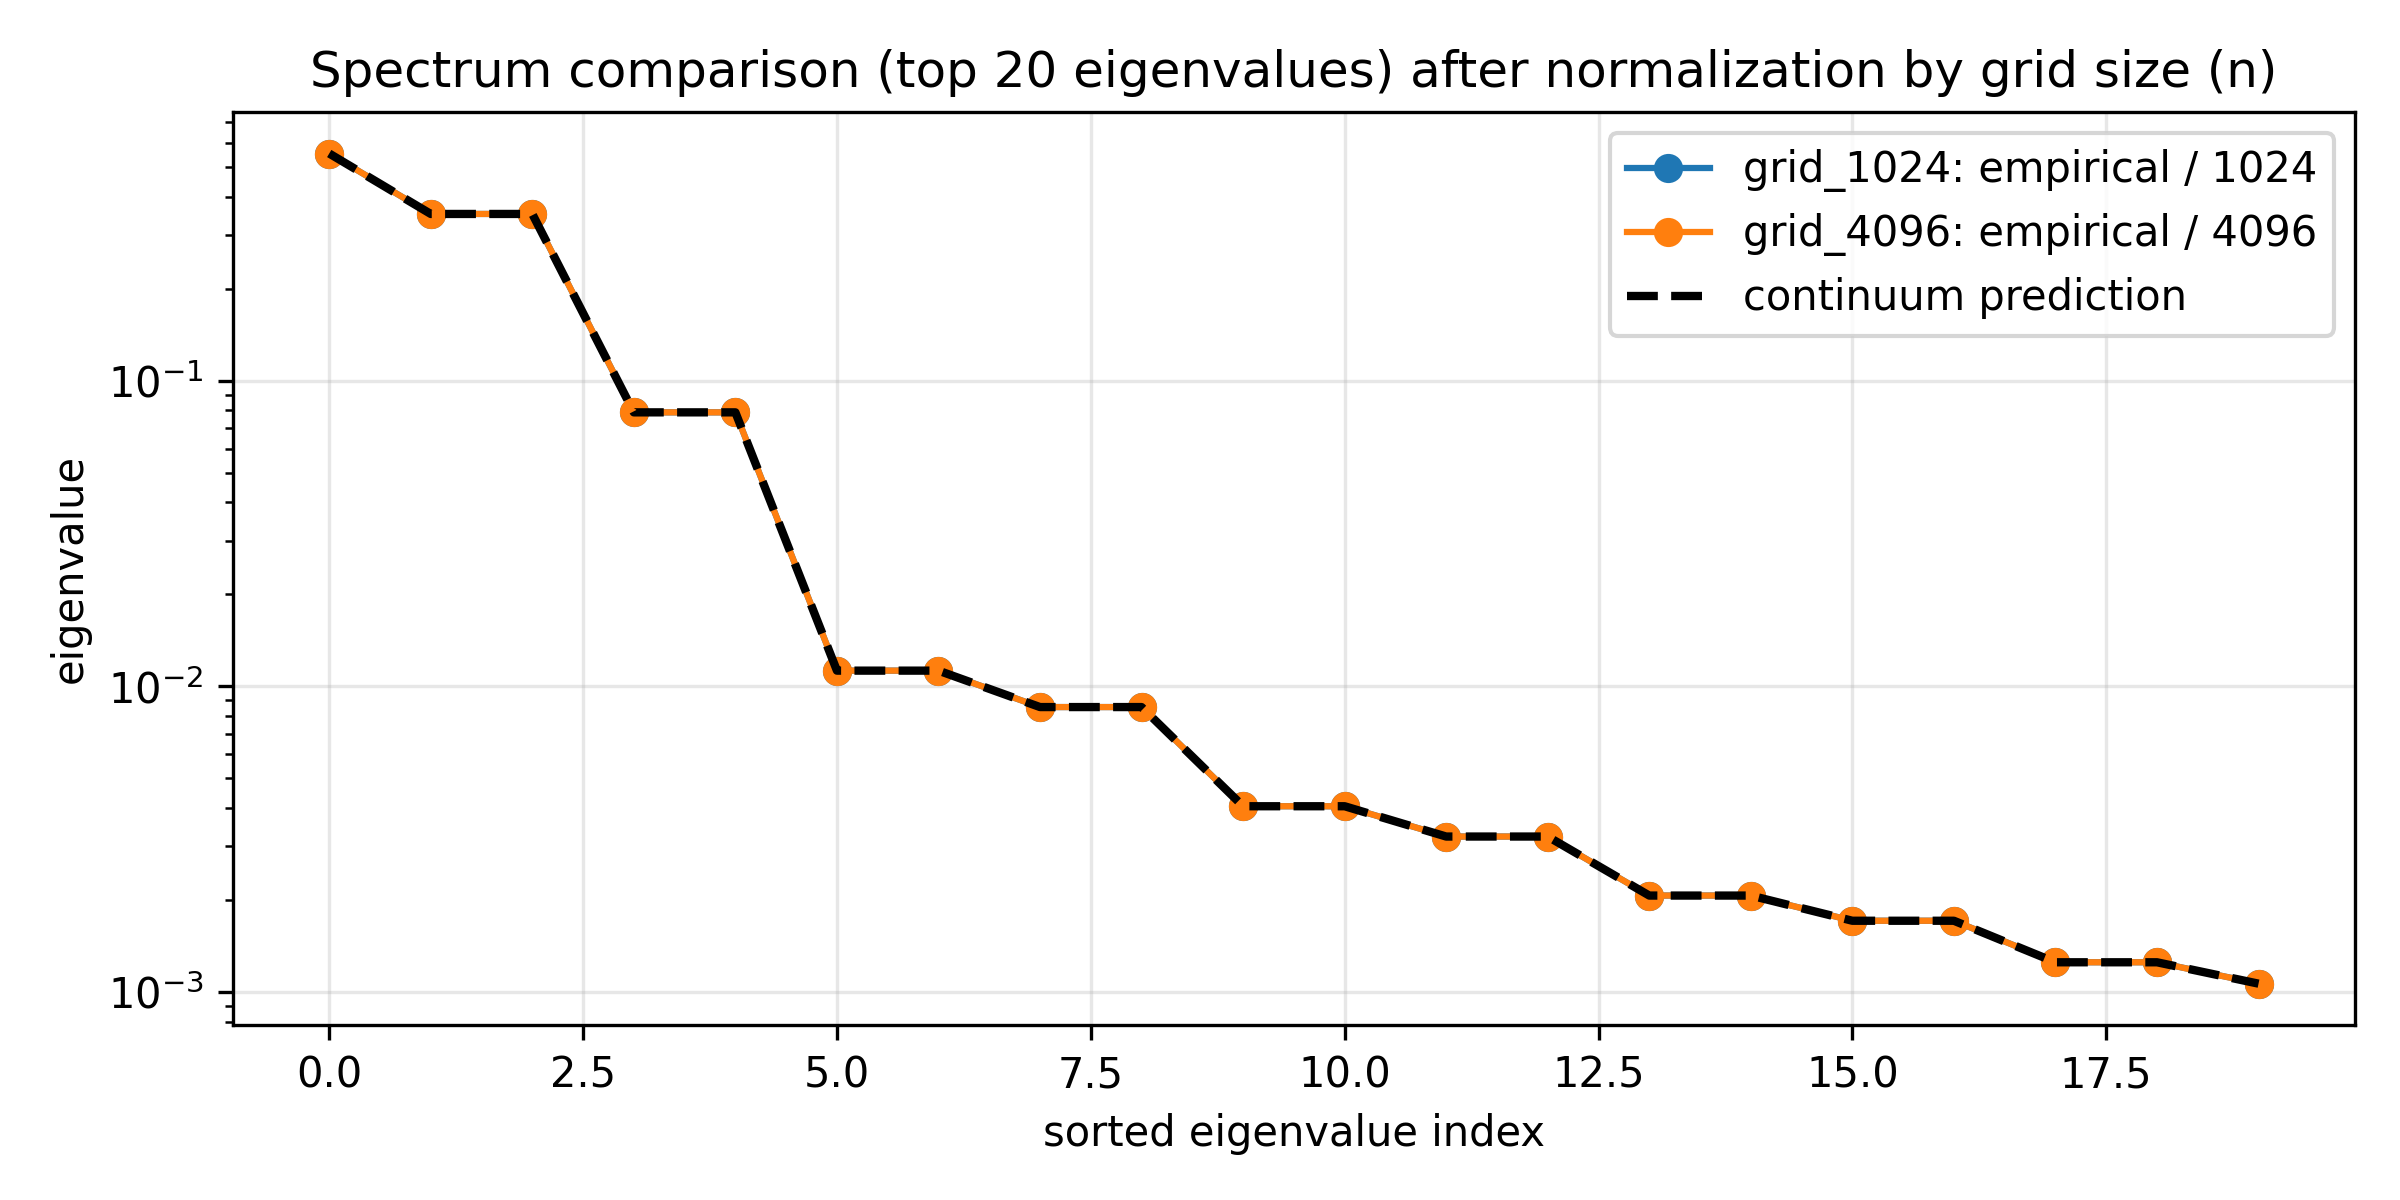
\includegraphics[width=0.7\textwidth]{images/spectrum_comparison_grid.png}
	\caption{Top empirical eigenvalues after normalization by grid size, compared with the continuum prediction.}
\end{figure}

\paragraph{Observations.}
\begin{itemize}
	\item After dividing by $n$, the empirical spectra for grid\_1024 and grid\_4096 are visually identical.
	\item Both empirical spectra match the continuum prediction extremely well.
	\item This indicates that, for the top modes at least, the $1024$-point grid is already a very accurate discretization of the continuum operator.
	\item Therefore, any remaining discrepancy in the time-domain plots is likely not caused by poor spectral approximation of the kernel itself.
\end{itemize}

\subsection*{Observed vs ideal normalized mode decay}

\begin{figure}[H]
	\centering
	\begin{subfigure}[t]{0.48\textwidth}
		\centering
		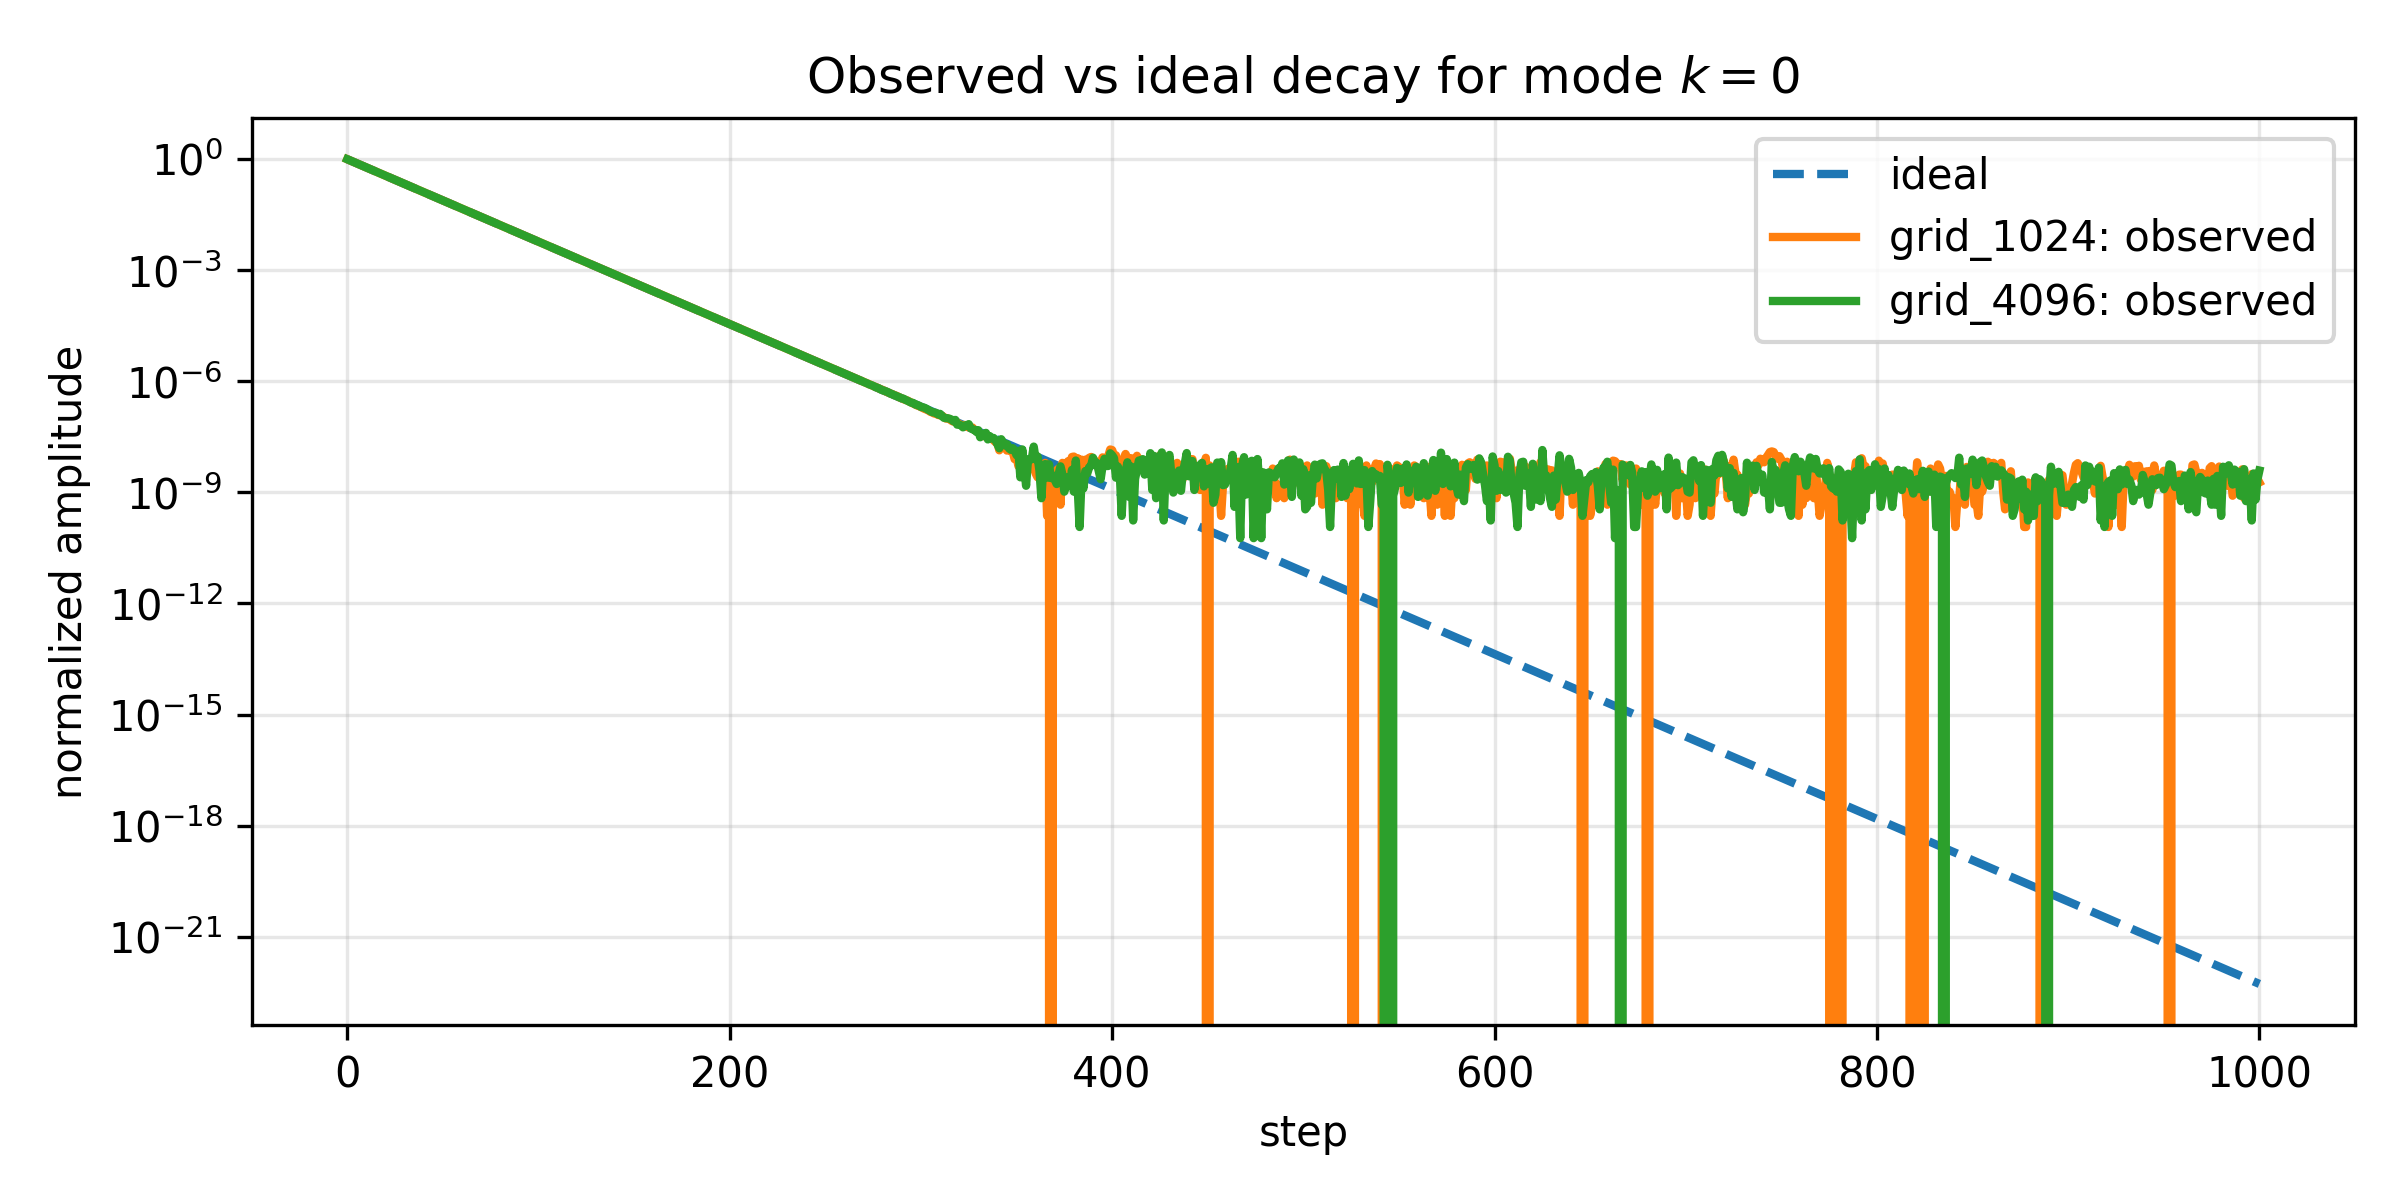
\includegraphics[width=\linewidth]{images/observed_vs_ideal_residual_decay_grid_mode_0.png}
		\caption{Mode $k=0$}
	\end{subfigure}
	\hfill
	\begin{subfigure}[t]{0.48\textwidth}
		\centering
		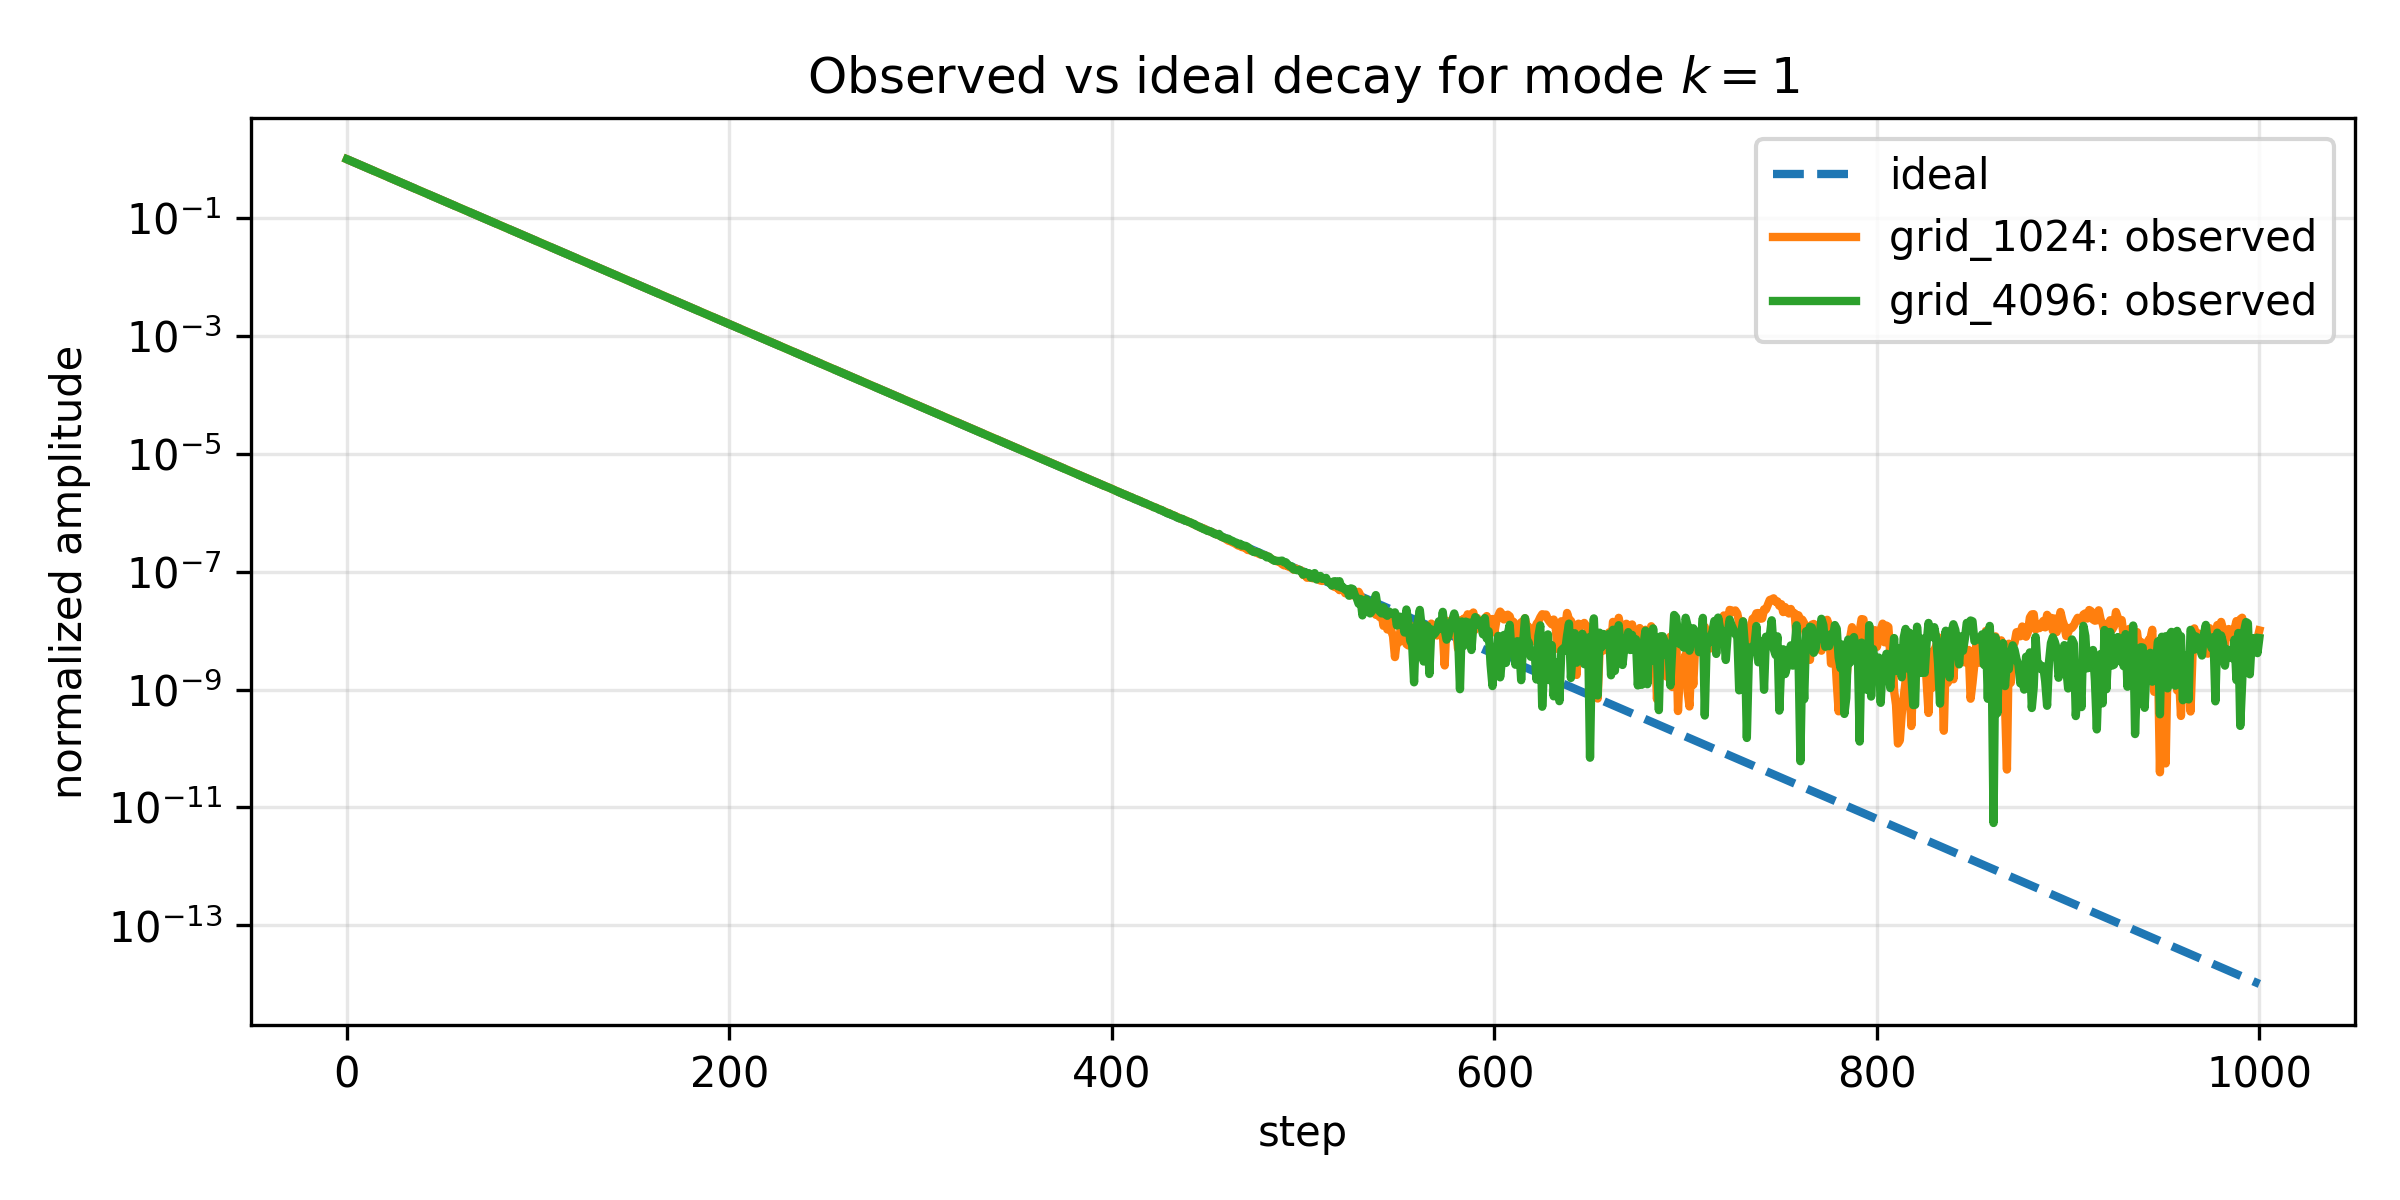
\includegraphics[width=\linewidth]{images/observed_vs_ideal_residual_decay_grid_mode_1.png}
		\caption{Mode $k=1$}
	\end{subfigure}

	\vspace{0.6em}

	\begin{subfigure}[t]{0.48\textwidth}
		\centering
		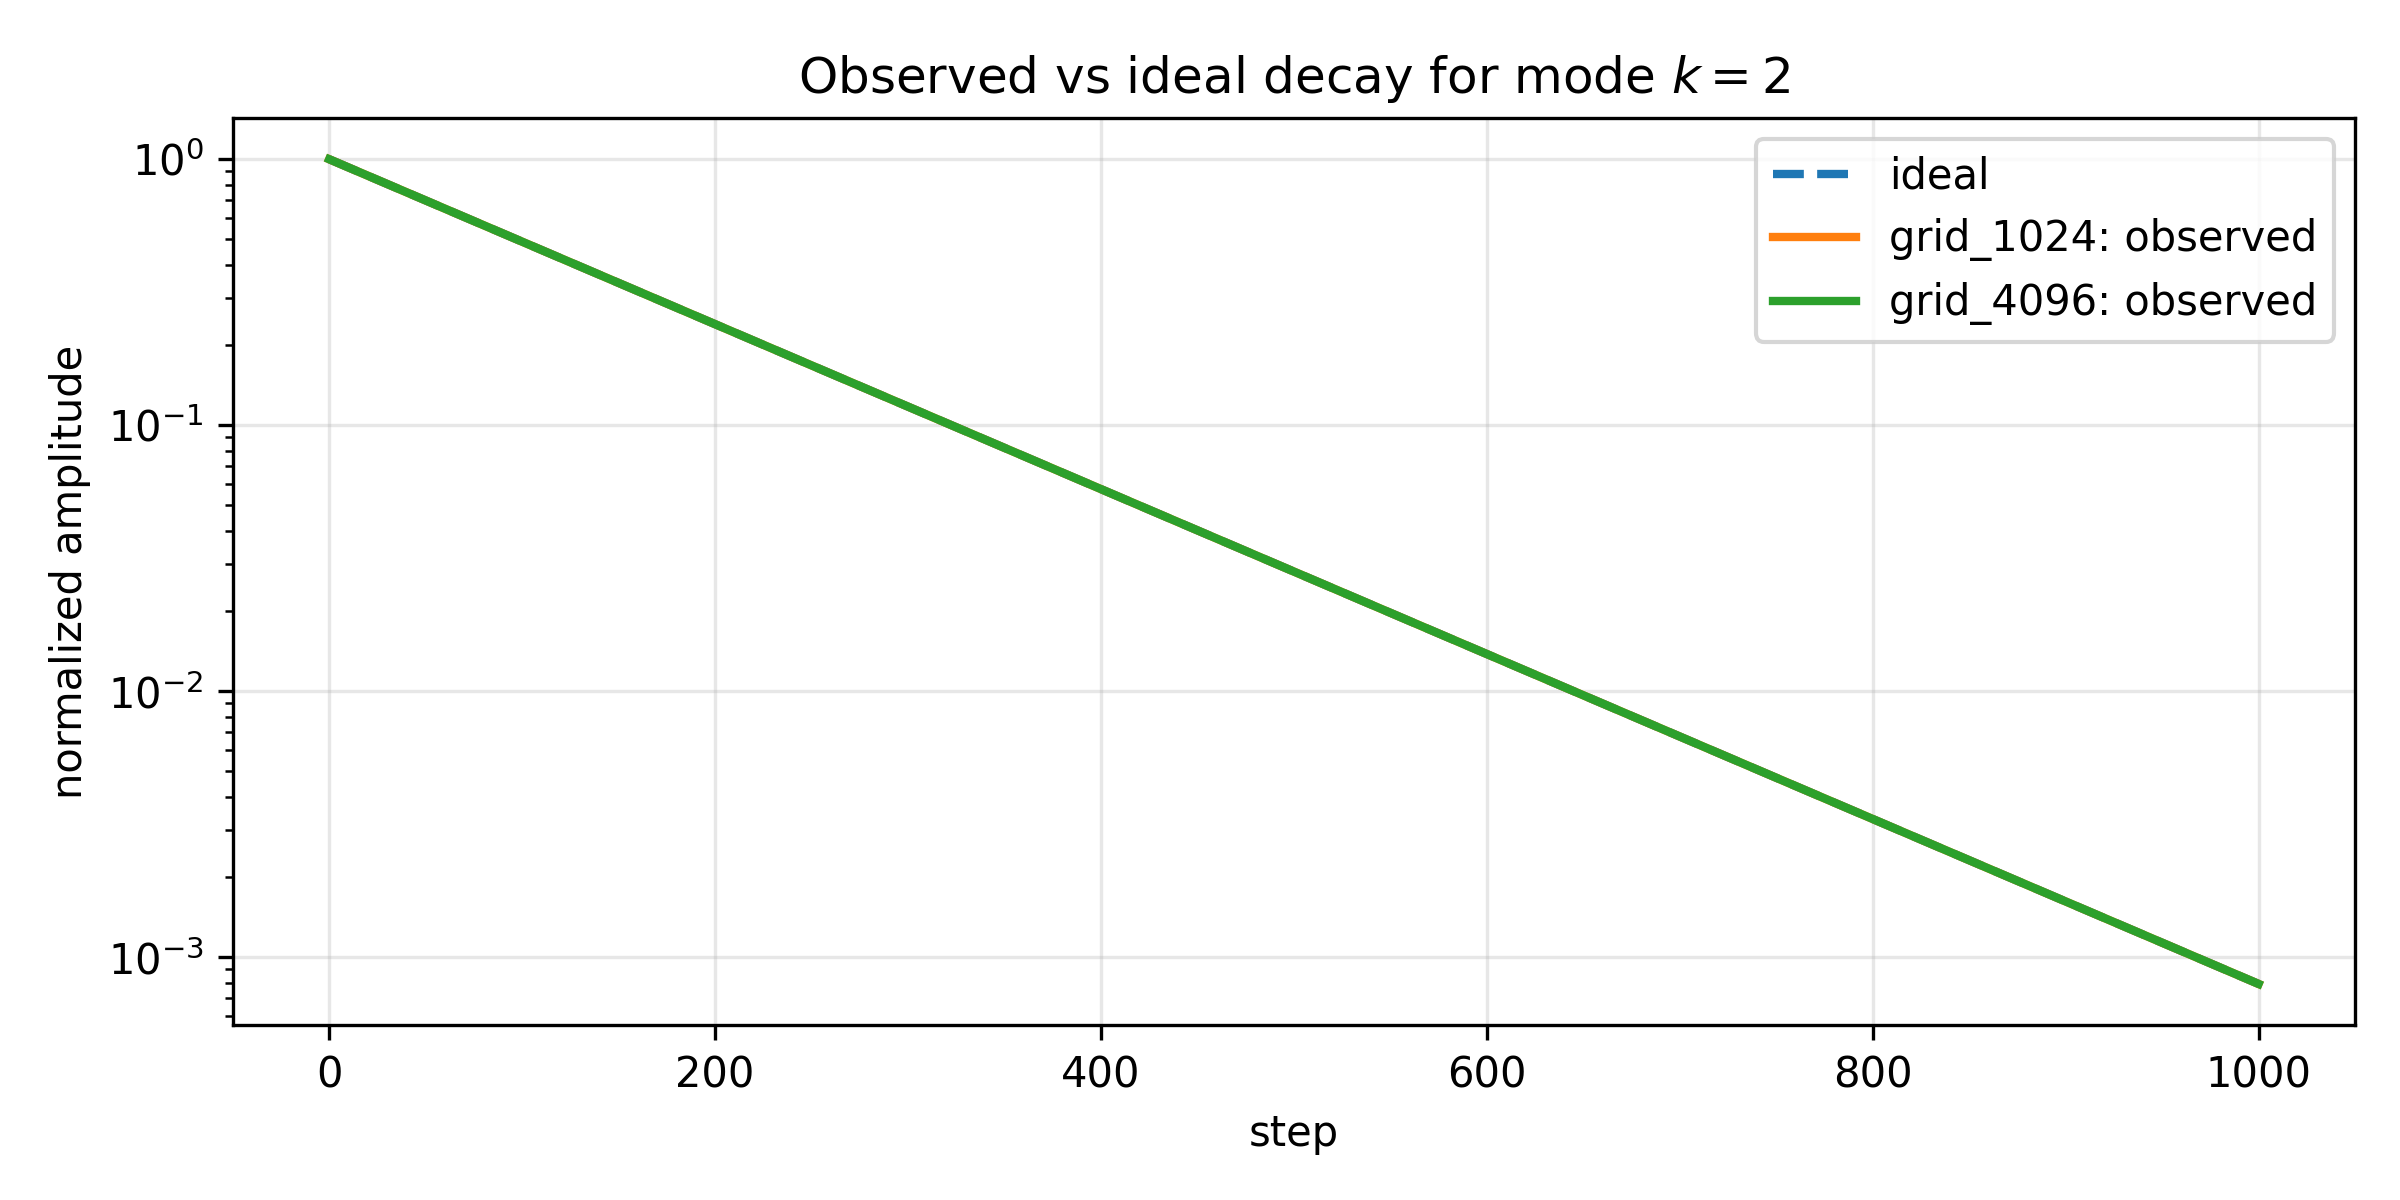
\includegraphics[width=\linewidth]{images/observed_vs_ideal_residual_decay_grid_mode_2.png}
		\caption{Mode $k=2$}
	\end{subfigure}
	\hfill
	\begin{subfigure}[t]{0.48\textwidth}
		\centering
		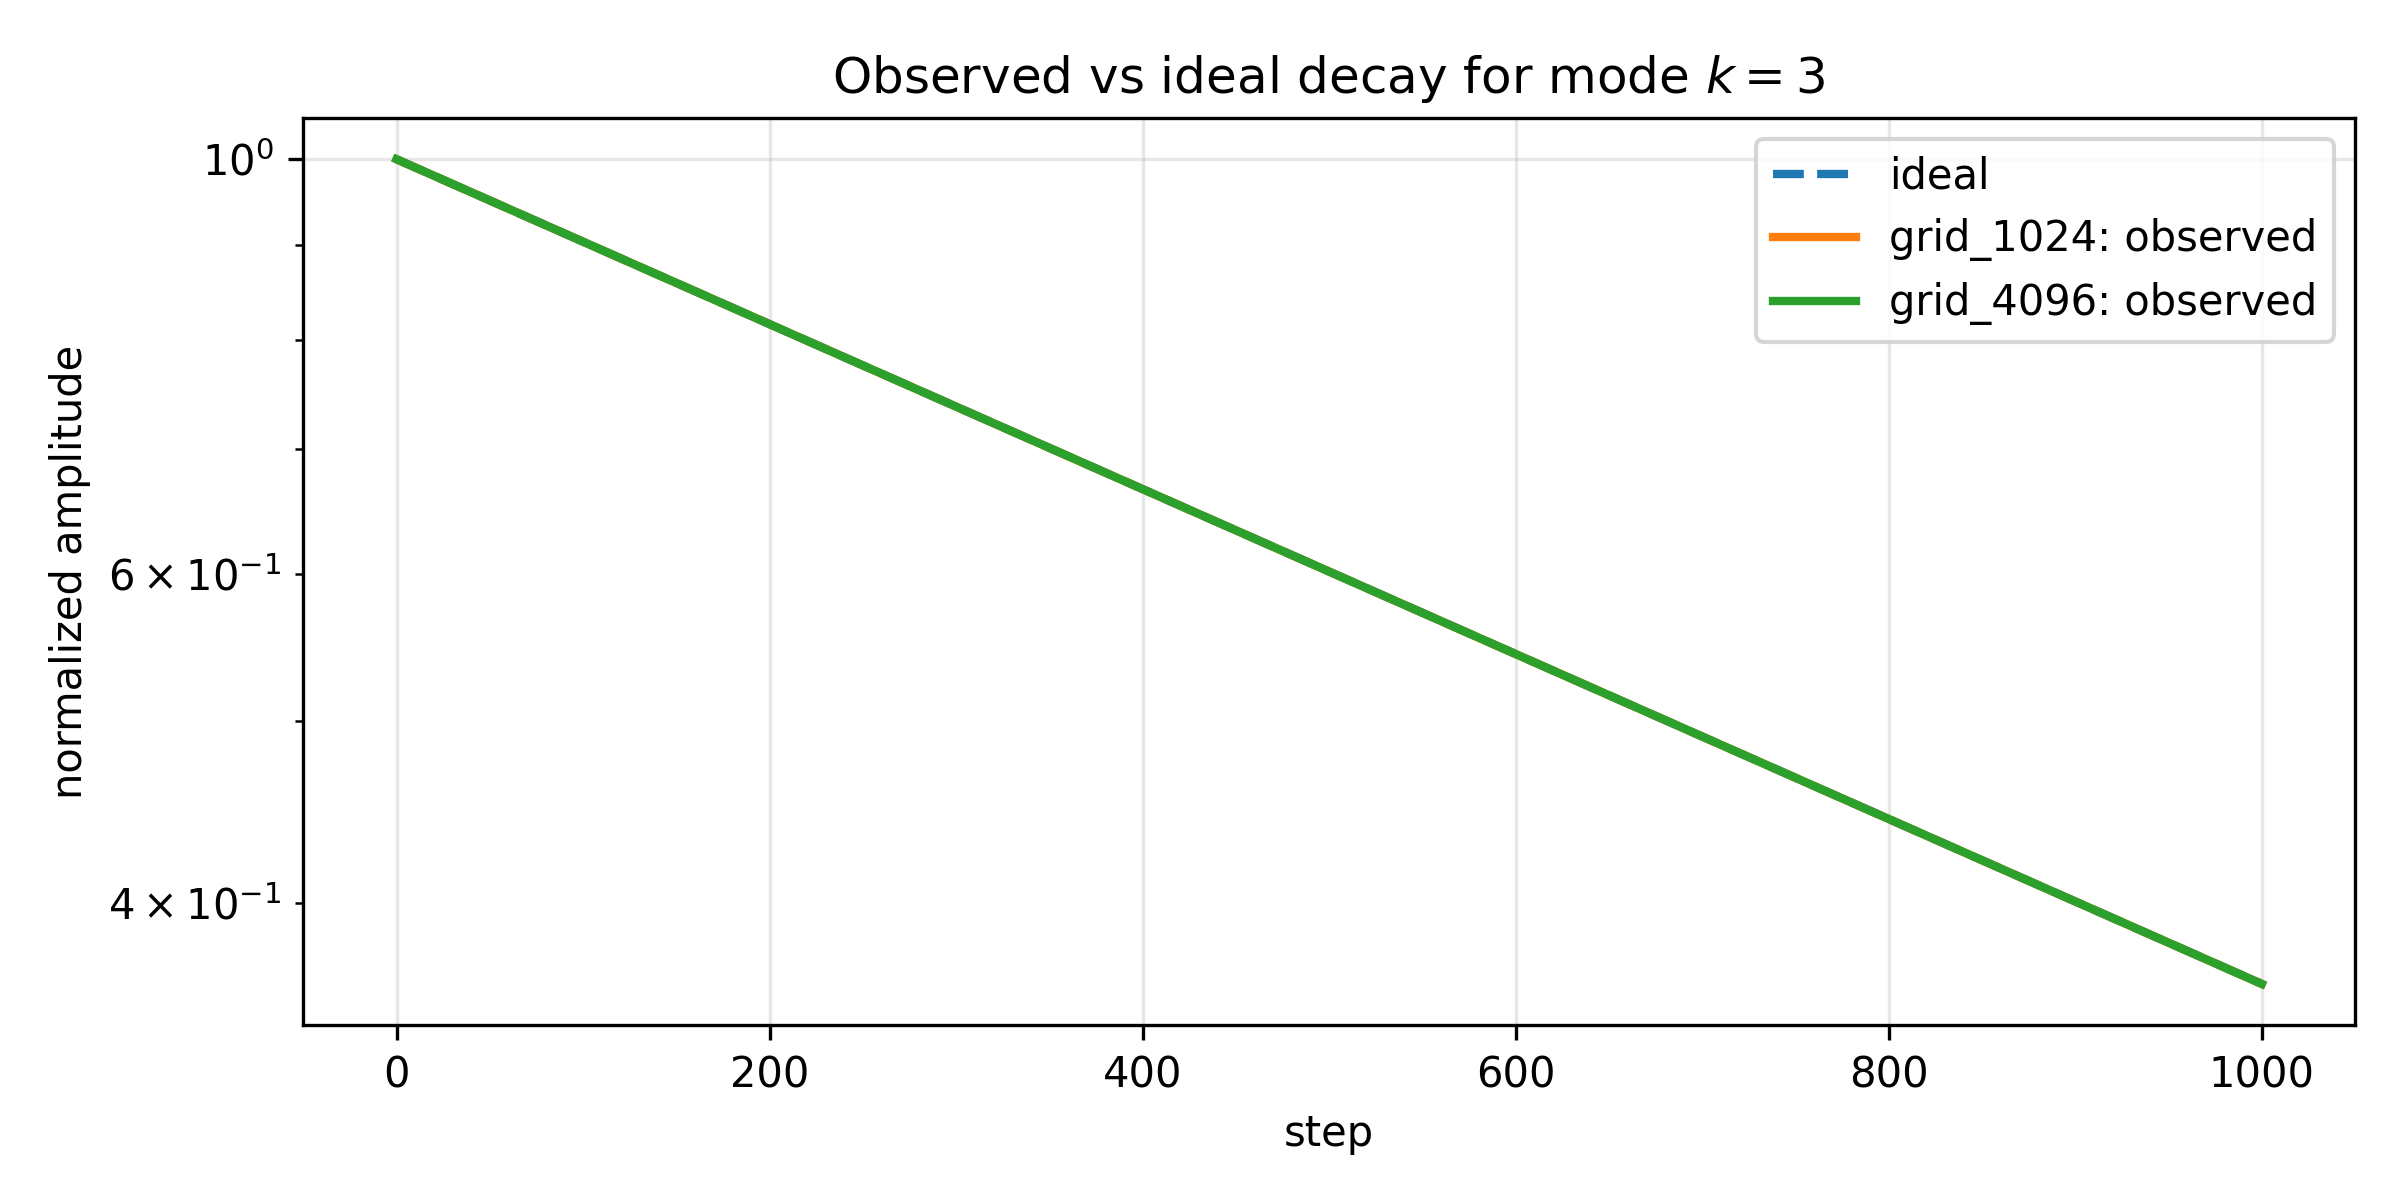
\includegraphics[width=\linewidth]{images/observed_vs_ideal_residual_decay_grid_mode_3.png}
		\caption{Mode $k=3$}
	\end{subfigure}
	\caption{Observed versus ideal normalized residual decay for modes $k=0,1,2,3$.}
\end{figure}

\paragraph{Observations.}
\begin{itemize}
	\item The decay rates are clearly ordered by mode: lower modes decay faster than higher modes, consistent with the spectral-bias picture.
	\item For modes $k=2$ and $k=3$, the observed normalized decay agrees essentially perfectly with the ideal prediction over the full time window.
	\item For modes $k=0$ and $k=1$, the observed curves initially agree with the ideal decay and then flatten once they hit the numerical floor.
	\item The flattening is therefore a numerical precision effect rather than a genuine deviation from the predicted dynamics.
	\item The two grid sizes behave almost identically in all four mode comparisons.
\end{itemize}

\section*{Conclusion}

The grid comparison leads to the following conclusions:
\begin{enumerate}
	\item The empirical kernel spectrum is already extremely well aligned with the continuum prediction at $n=1024$.
	\item Increasing the grid from $1024$ to $4096$ does not materially change the fitted function, the normalized loss curve, or the normalized mode decay.
	\item The dominant discrepancy in the slow modes is not caused by the discretization, but by the finite time horizon and numerical precision effects.
	\item The mode-wise decay remains fully consistent with the formula
	      \[
		      r_k(t) = (1-\eta\lambda_k^{\mathrm{emp}})^t r_k(0).
	      \]
\end{enumerate}

In particular, the finer-grid experiment suggests that the $1024$-point equally spaced grid is a sufficient approximation.

\section*{Results: baseline target vs high-frequency-heavy target}

We now compare two experiments on the same equally spaced grid ($1024$ points), with the same kernel and the same active frequencies, but with different amplitudes:

\[
	\text{baseline: }
	y(\gamma)=1+0.9\cos(\gamma)+0.5\cos(2\gamma)+0.35\cos(3\gamma),
\]
\[
	\text{highfreq\_heavy: }
	y(\gamma)=1+0.35\cos(\gamma)+0.9\cos(2\gamma)+1.4\cos(3\gamma).
\]

The goal of this comparison is to check whether changing amplitudes changes the \emph{decay rates} of the modes.
For standard kernel GD, the prediction is that the normalized decay curves should be unchanged, since the decay rate is controlled by the eigenvalues and not by the amplitudes.

\subsection*{Target functions and final predictions}

\begin{figure}[H]
	\centering
	\begin{subfigure}[t]{0.48\textwidth}
		\centering
		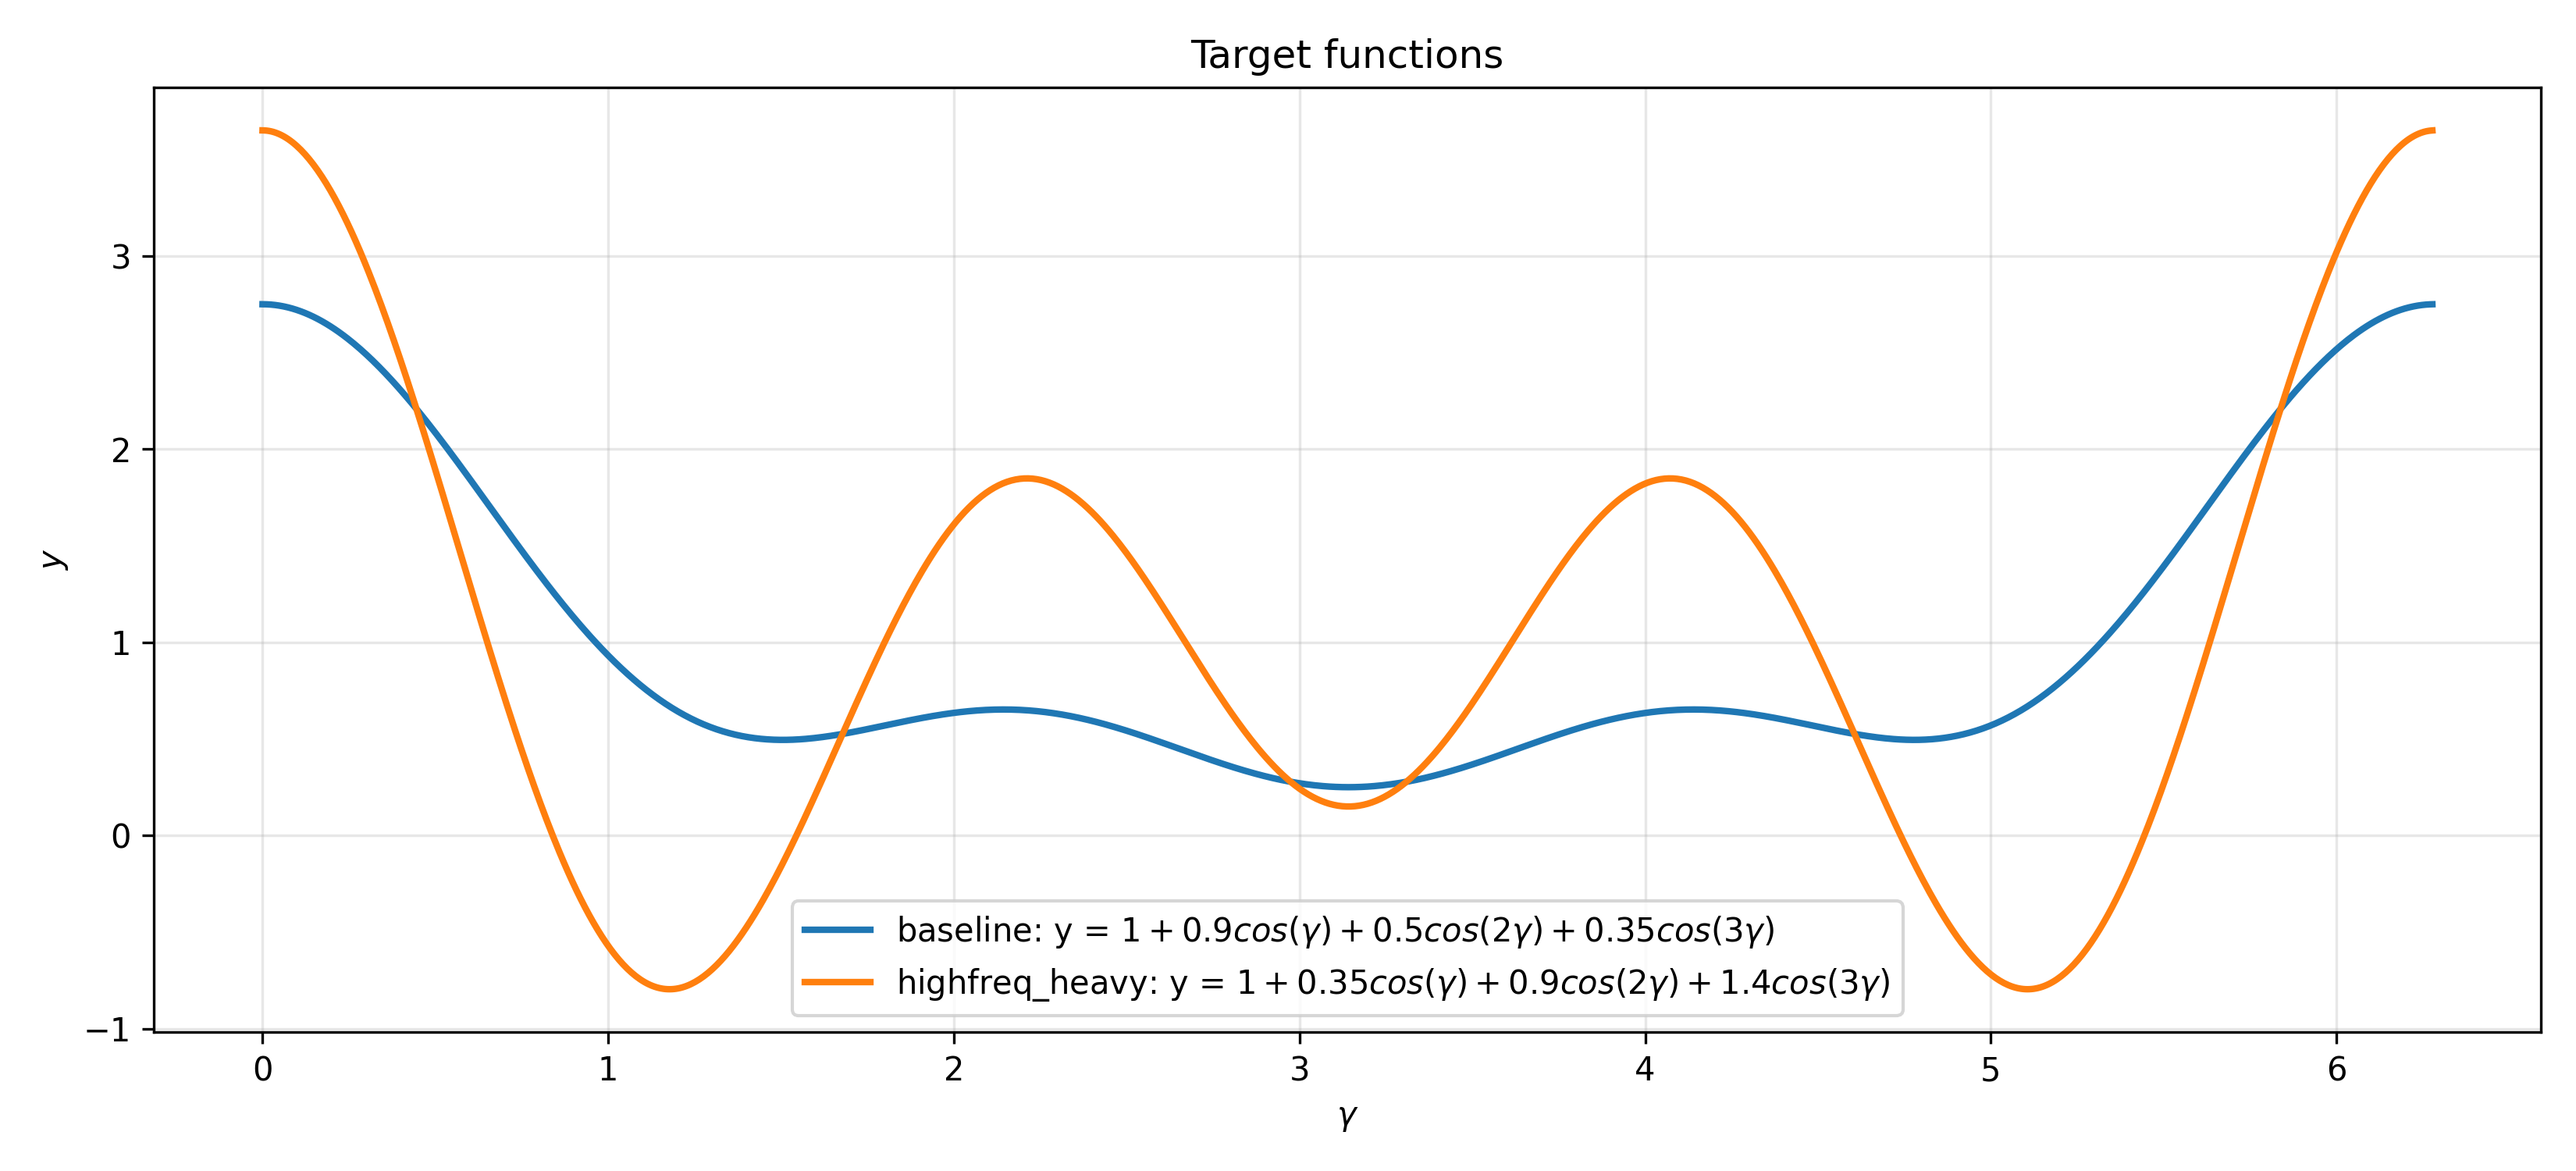
\includegraphics[width=\linewidth]{images/target_functions.png}
		\caption{Baseline and high-frequency-heavy targets}
	\end{subfigure}
	\hfill
	\begin{subfigure}[t]{0.48\textwidth}
		\centering
		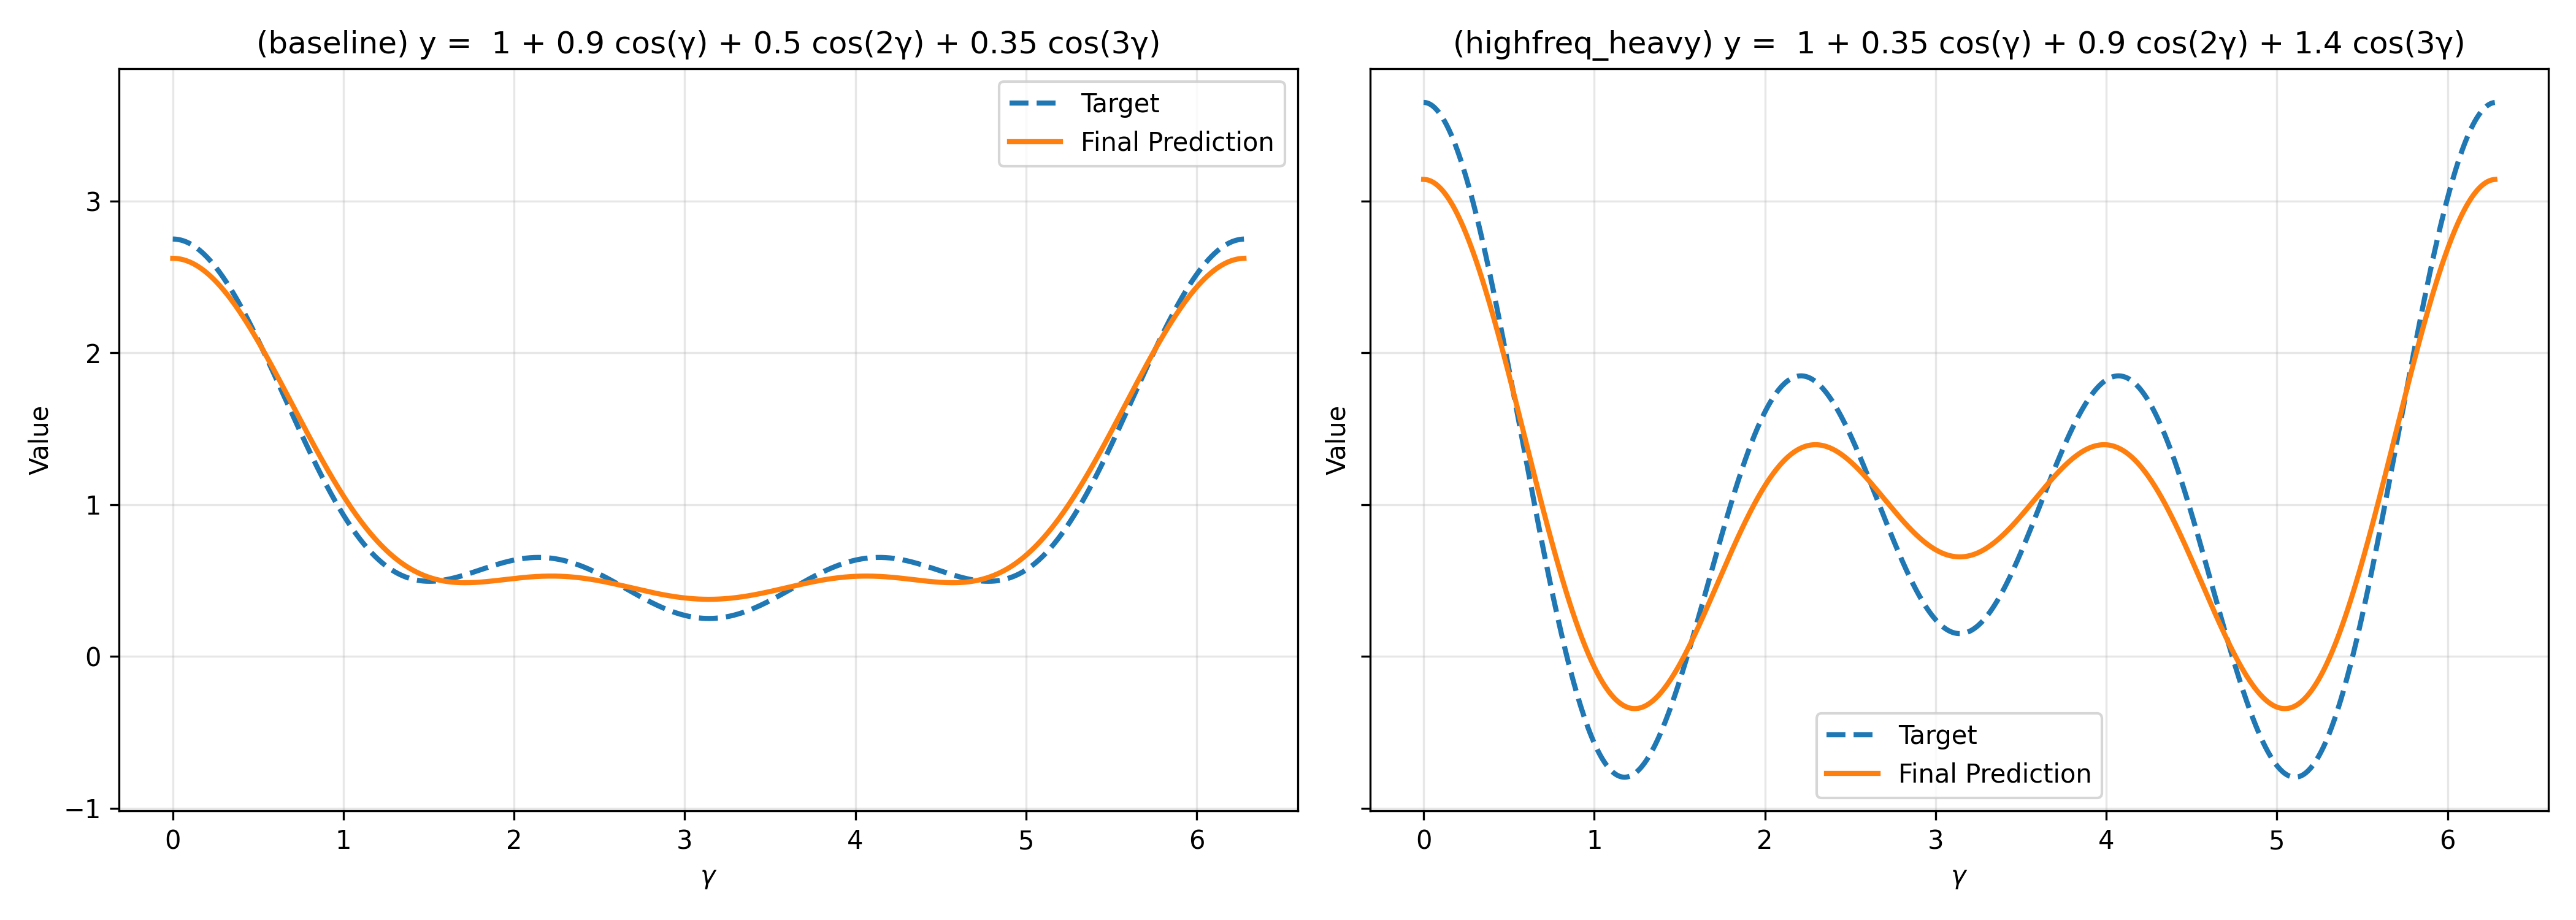
\includegraphics[width=\linewidth]{images/final_predictions_baseline_vs_highfreq.png}
		\caption{Final predictions for both targets}
	\end{subfigure}
	\caption{Comparison of the two target functions and their final fitted predictions.}
\end{figure}

\paragraph{Observations.}
\begin{itemize}
	\item The high-frequency-heavy target has substantially more oscillatory structure than the baseline target.
	\item After the same number of GD steps, the baseline target is fitted noticeably better than the high-frequency-heavy target.
	\item The final prediction for the high-frequency-heavy case is visibly smoother than the target, which indicates underfitting of the higher-frequency content.
	\item This is consistent with spectral bias: the larger high-frequency amplitude in the target does not make that mode learn faster.
\end{itemize}

\subsection*{Relative residual decay}

\begin{figure}[H]
	\centering
	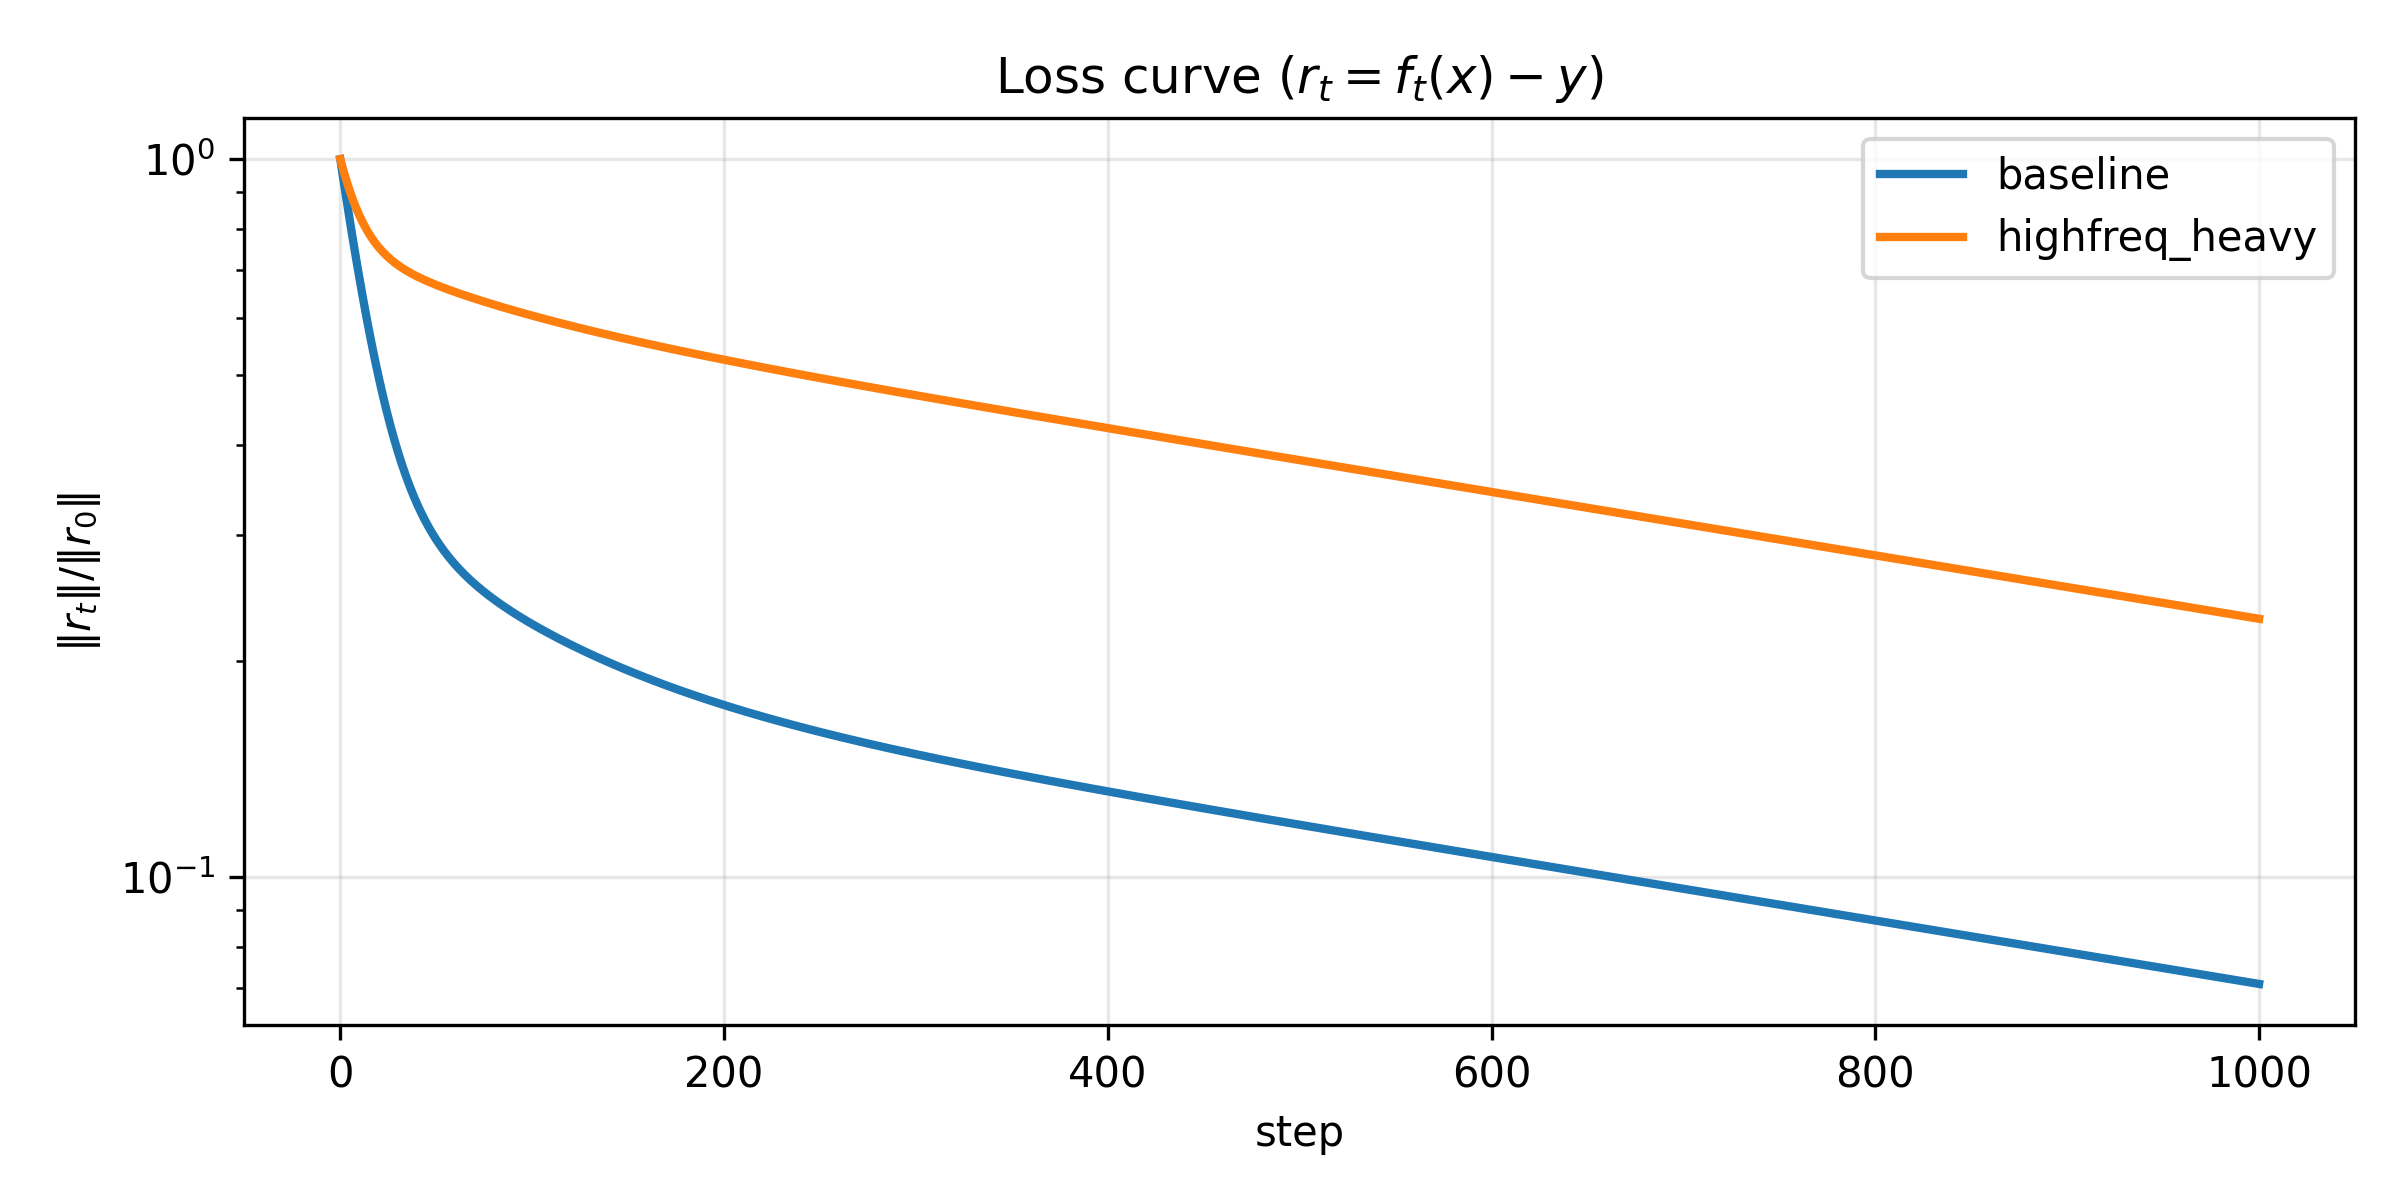
\includegraphics[width=0.68\textwidth]{images/loss_curve_baseline_vs_highfreq.png}
	\caption{Relative residual decay for the baseline and high-frequency-heavy targets.}
\end{figure}

\paragraph{Observations.}
\begin{itemize}
	\item The high-frequency-heavy experiment decays more slowly in relative residual norm.
	\item This is not because the kernel dynamics changed, but because a larger fraction of the initial target energy is placed in the slower modes.
	\item In particular, increasing the amplitude of the $k=3$ mode makes the overall fit look worse at finite time, even though the per-mode rates are unchanged.
\end{itemize}

\subsection*{Final prediction error}

\begin{figure}[H]
	\centering
	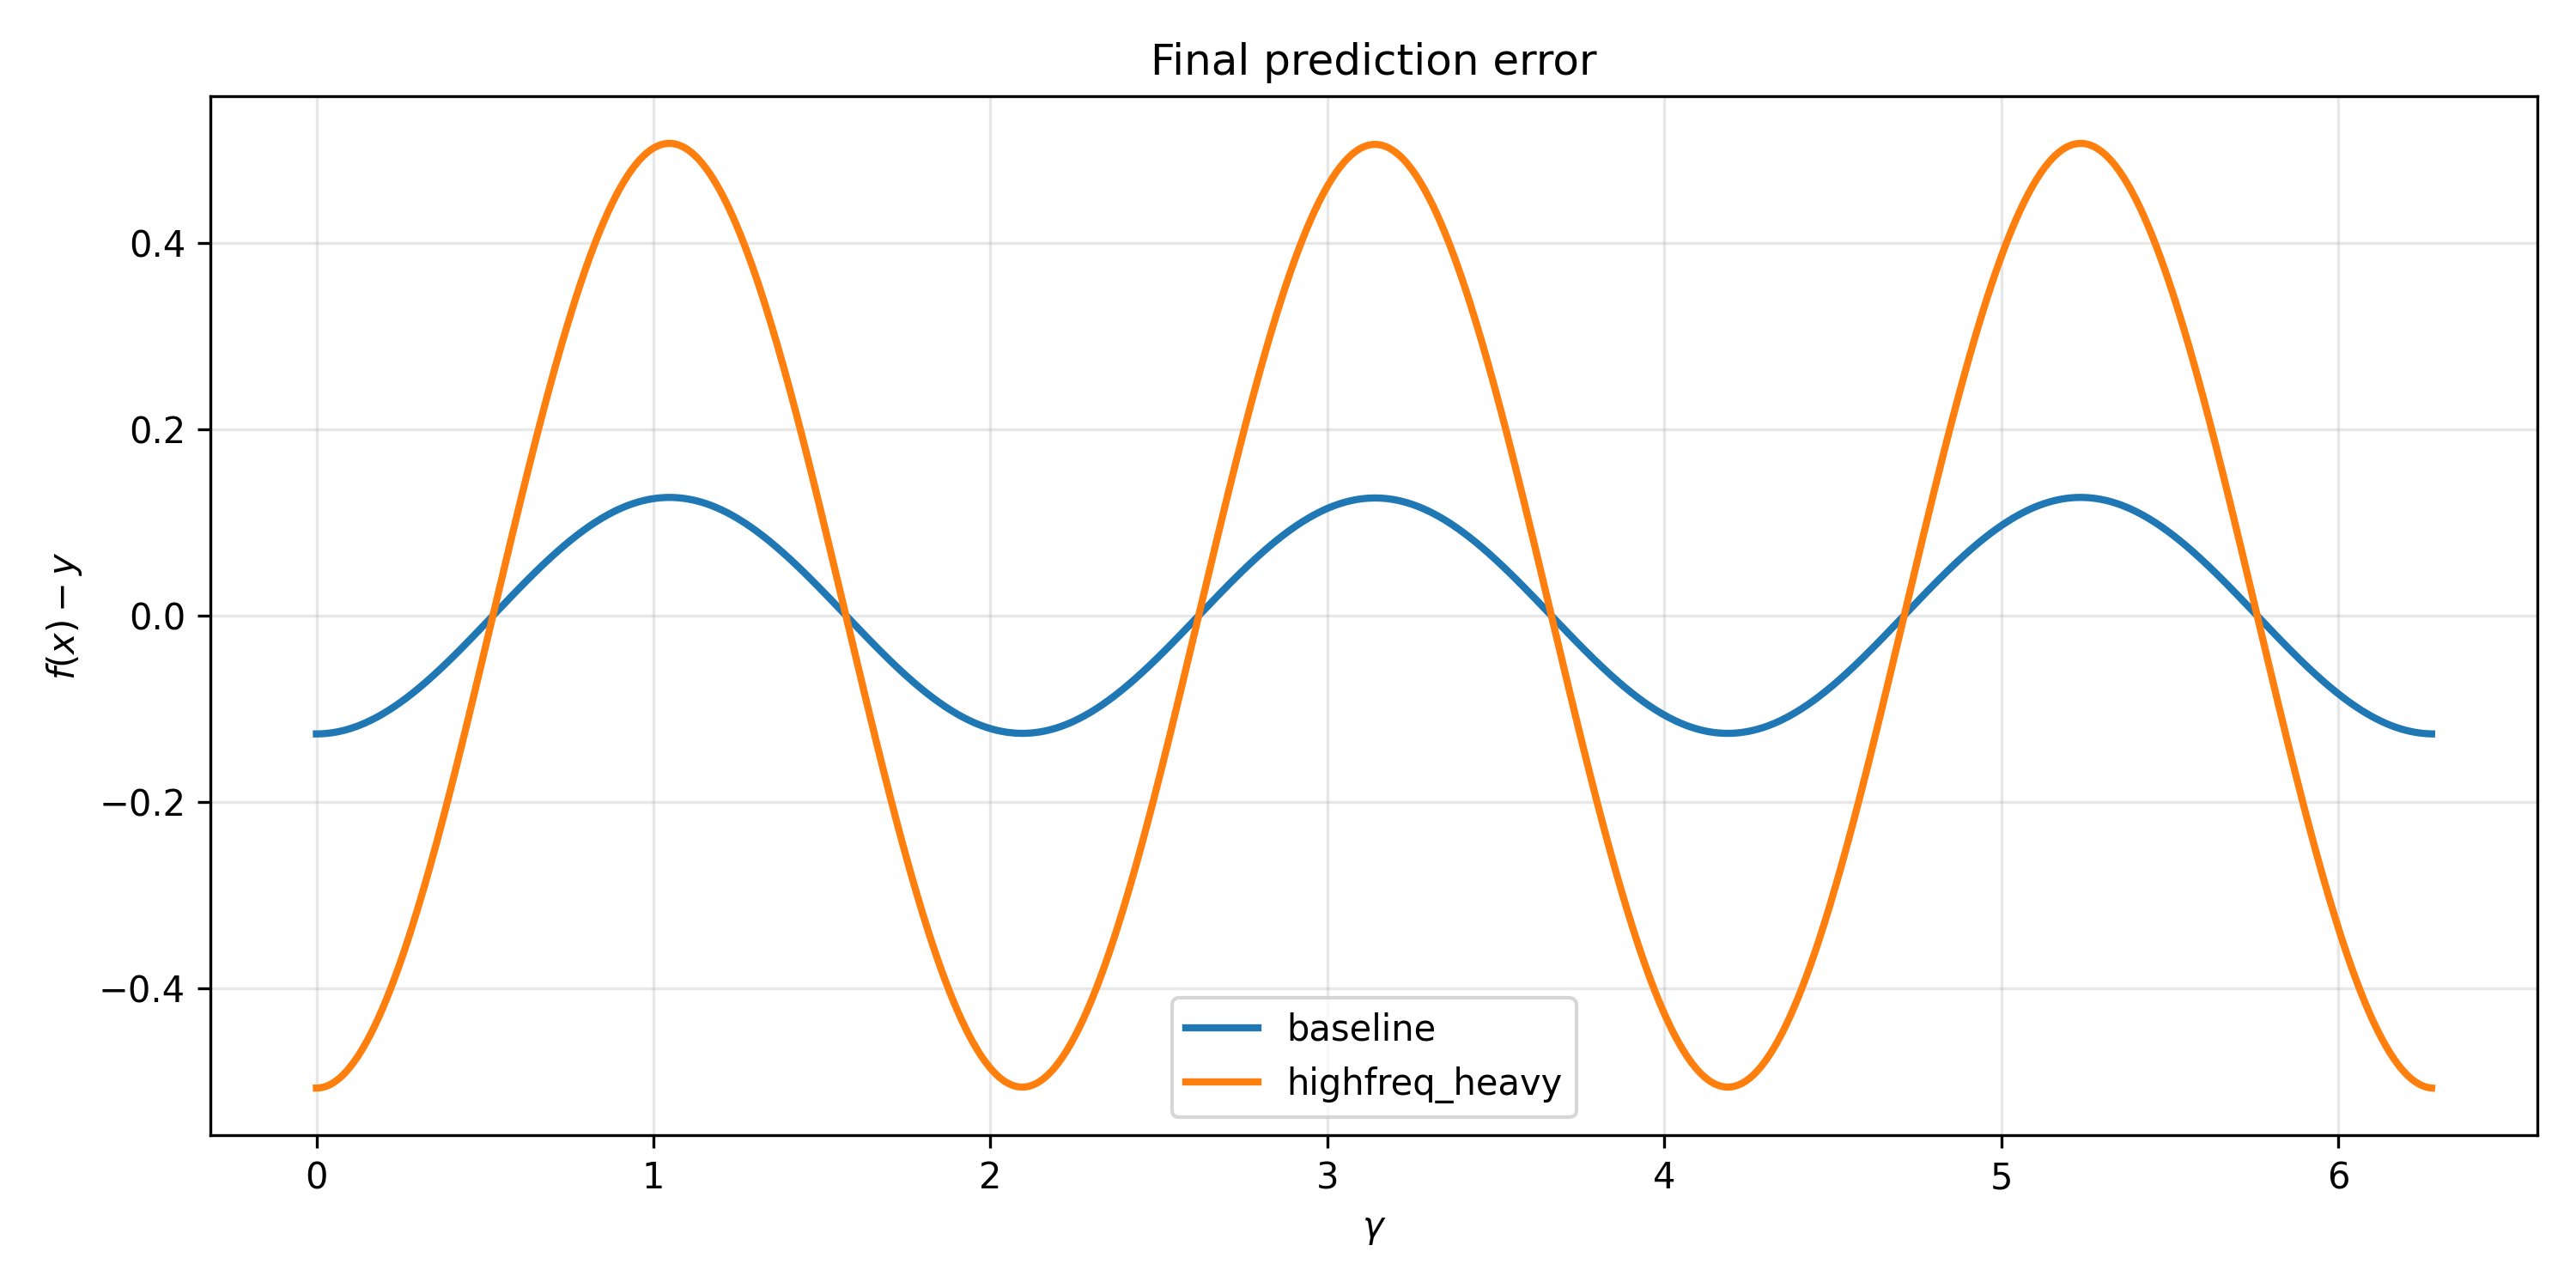
\includegraphics[width=0.7\textwidth]{images/prediction_error_high_frequency.png}
	\caption{Final prediction error $f(x)-y$ for the baseline and high-frequency-heavy targets.}
\end{figure}

\paragraph{Observations.}
\begin{itemize}
	\item The final prediction error is substantially larger for the high-frequency-heavy target than for the baseline target.
	\item In both cases the error is highly structured and oscillatory rather than random, indicating that the remaining error is concentrated in unresolved Fourier modes.
	\item The high-frequency-heavy target places much more mass in the slower modes, especially $k=2$ and $k=3$, so after the same number of GD steps those components remain more visible in the final error.
	\item This is consistent with the mode-wise analysis: the normalized decay rates are unchanged, but the absolute residual is larger because more target energy lies in modes with smaller eigenvalues.
\end{itemize}

\subsection*{Observed vs ideal normalized mode decay}

\begin{figure}[H]
	\centering
	\begin{subfigure}[t]{0.48\textwidth}
		\centering
		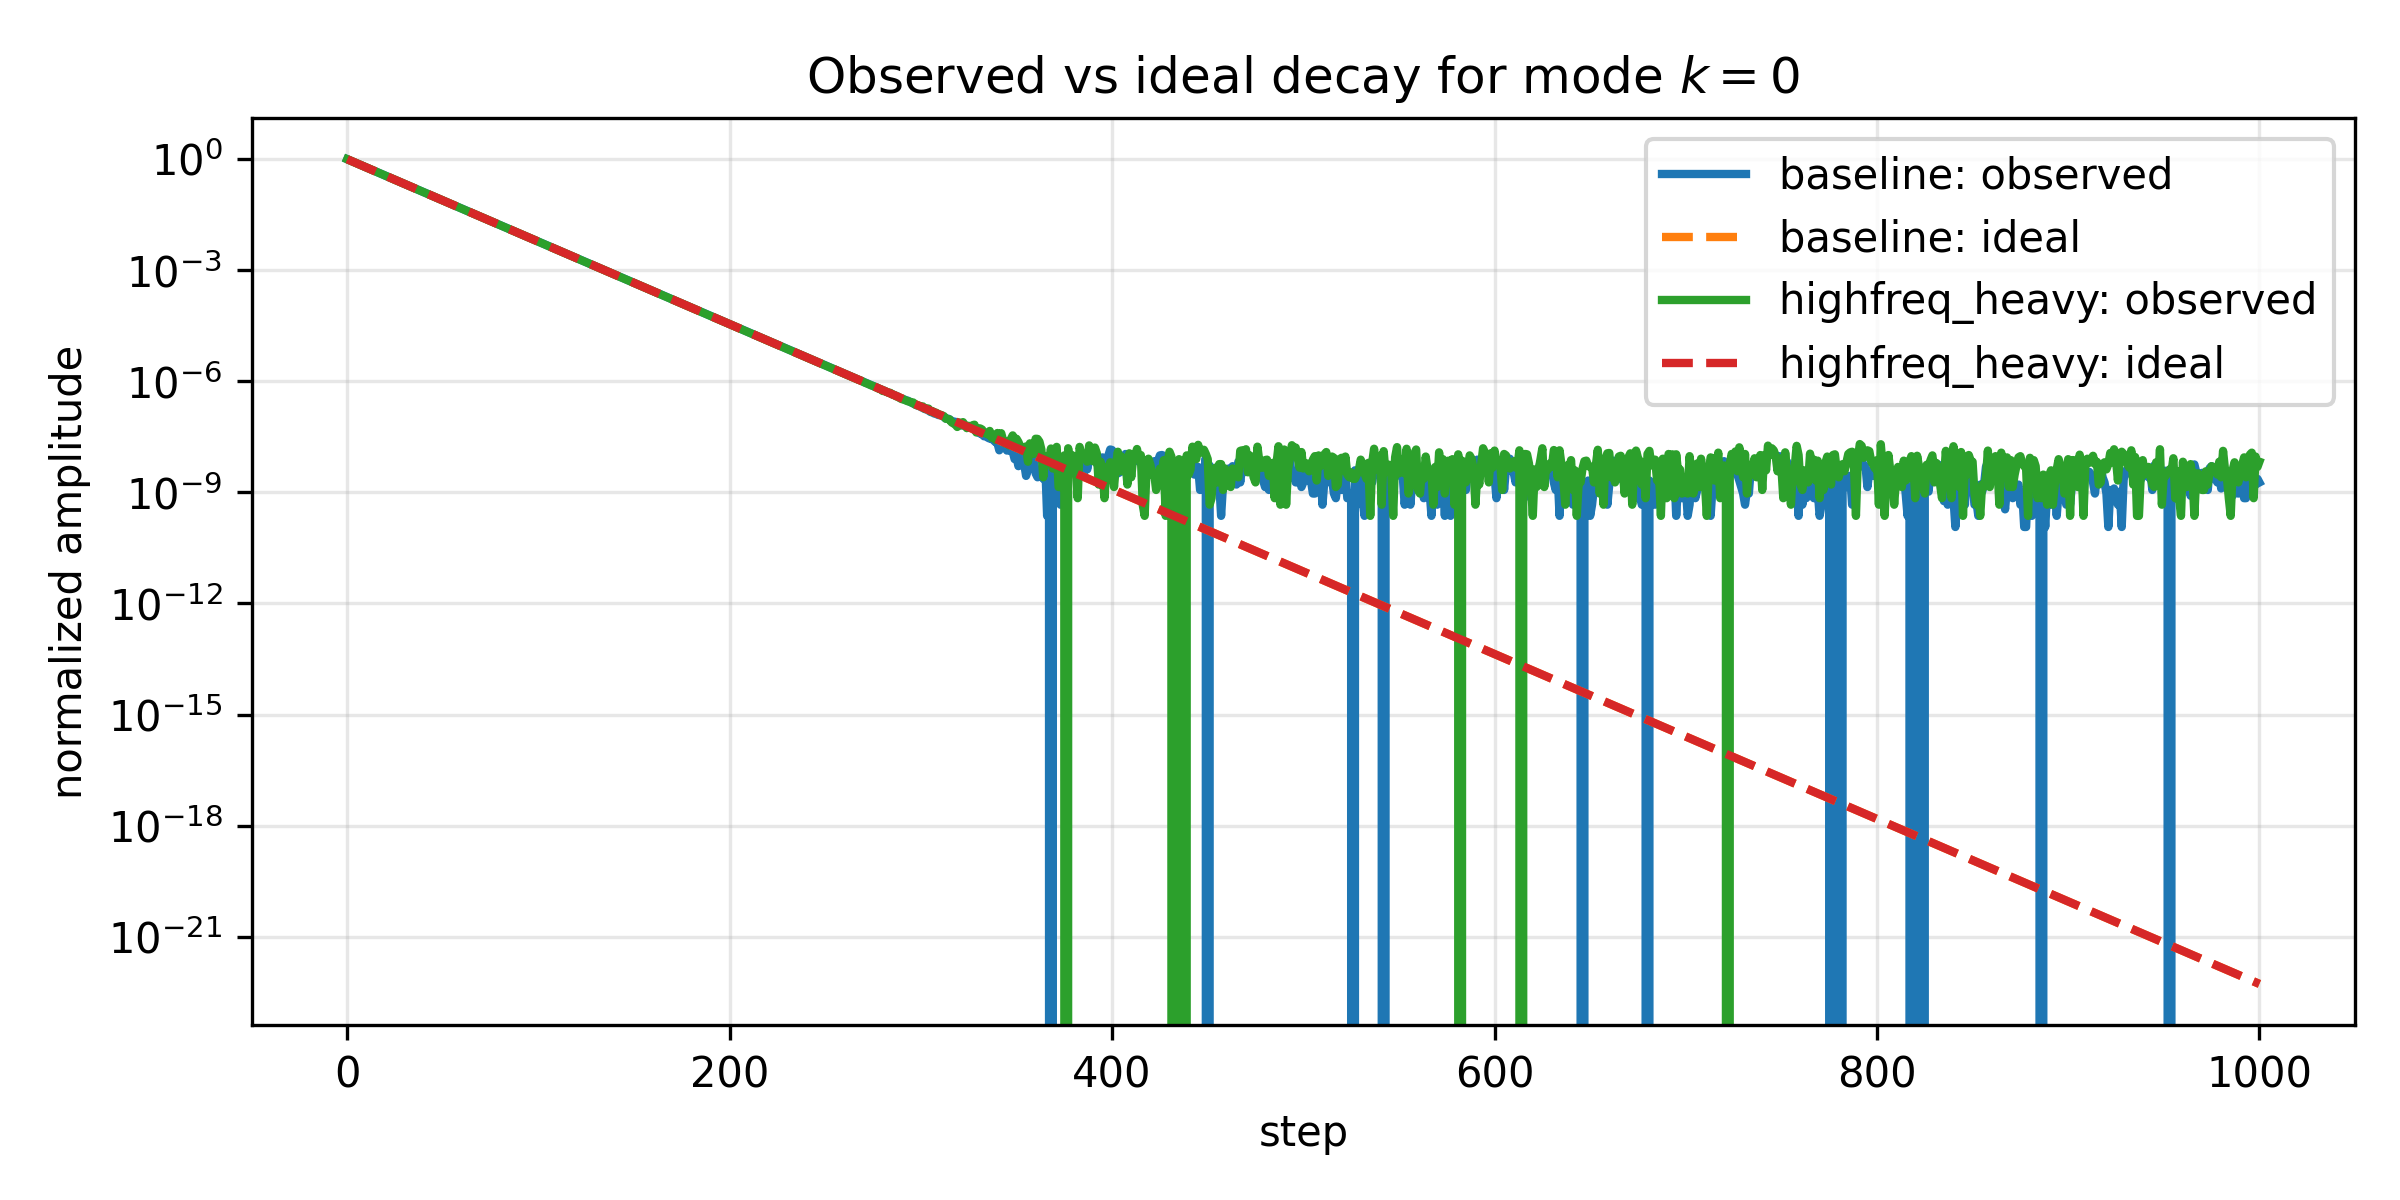
\includegraphics[width=\linewidth]{images/observed_vs_ideal_residual_decay_mode_0.png}
		\caption{Mode $k=0$}
	\end{subfigure}
	\hfill
	\begin{subfigure}[t]{0.48\textwidth}
		\centering
		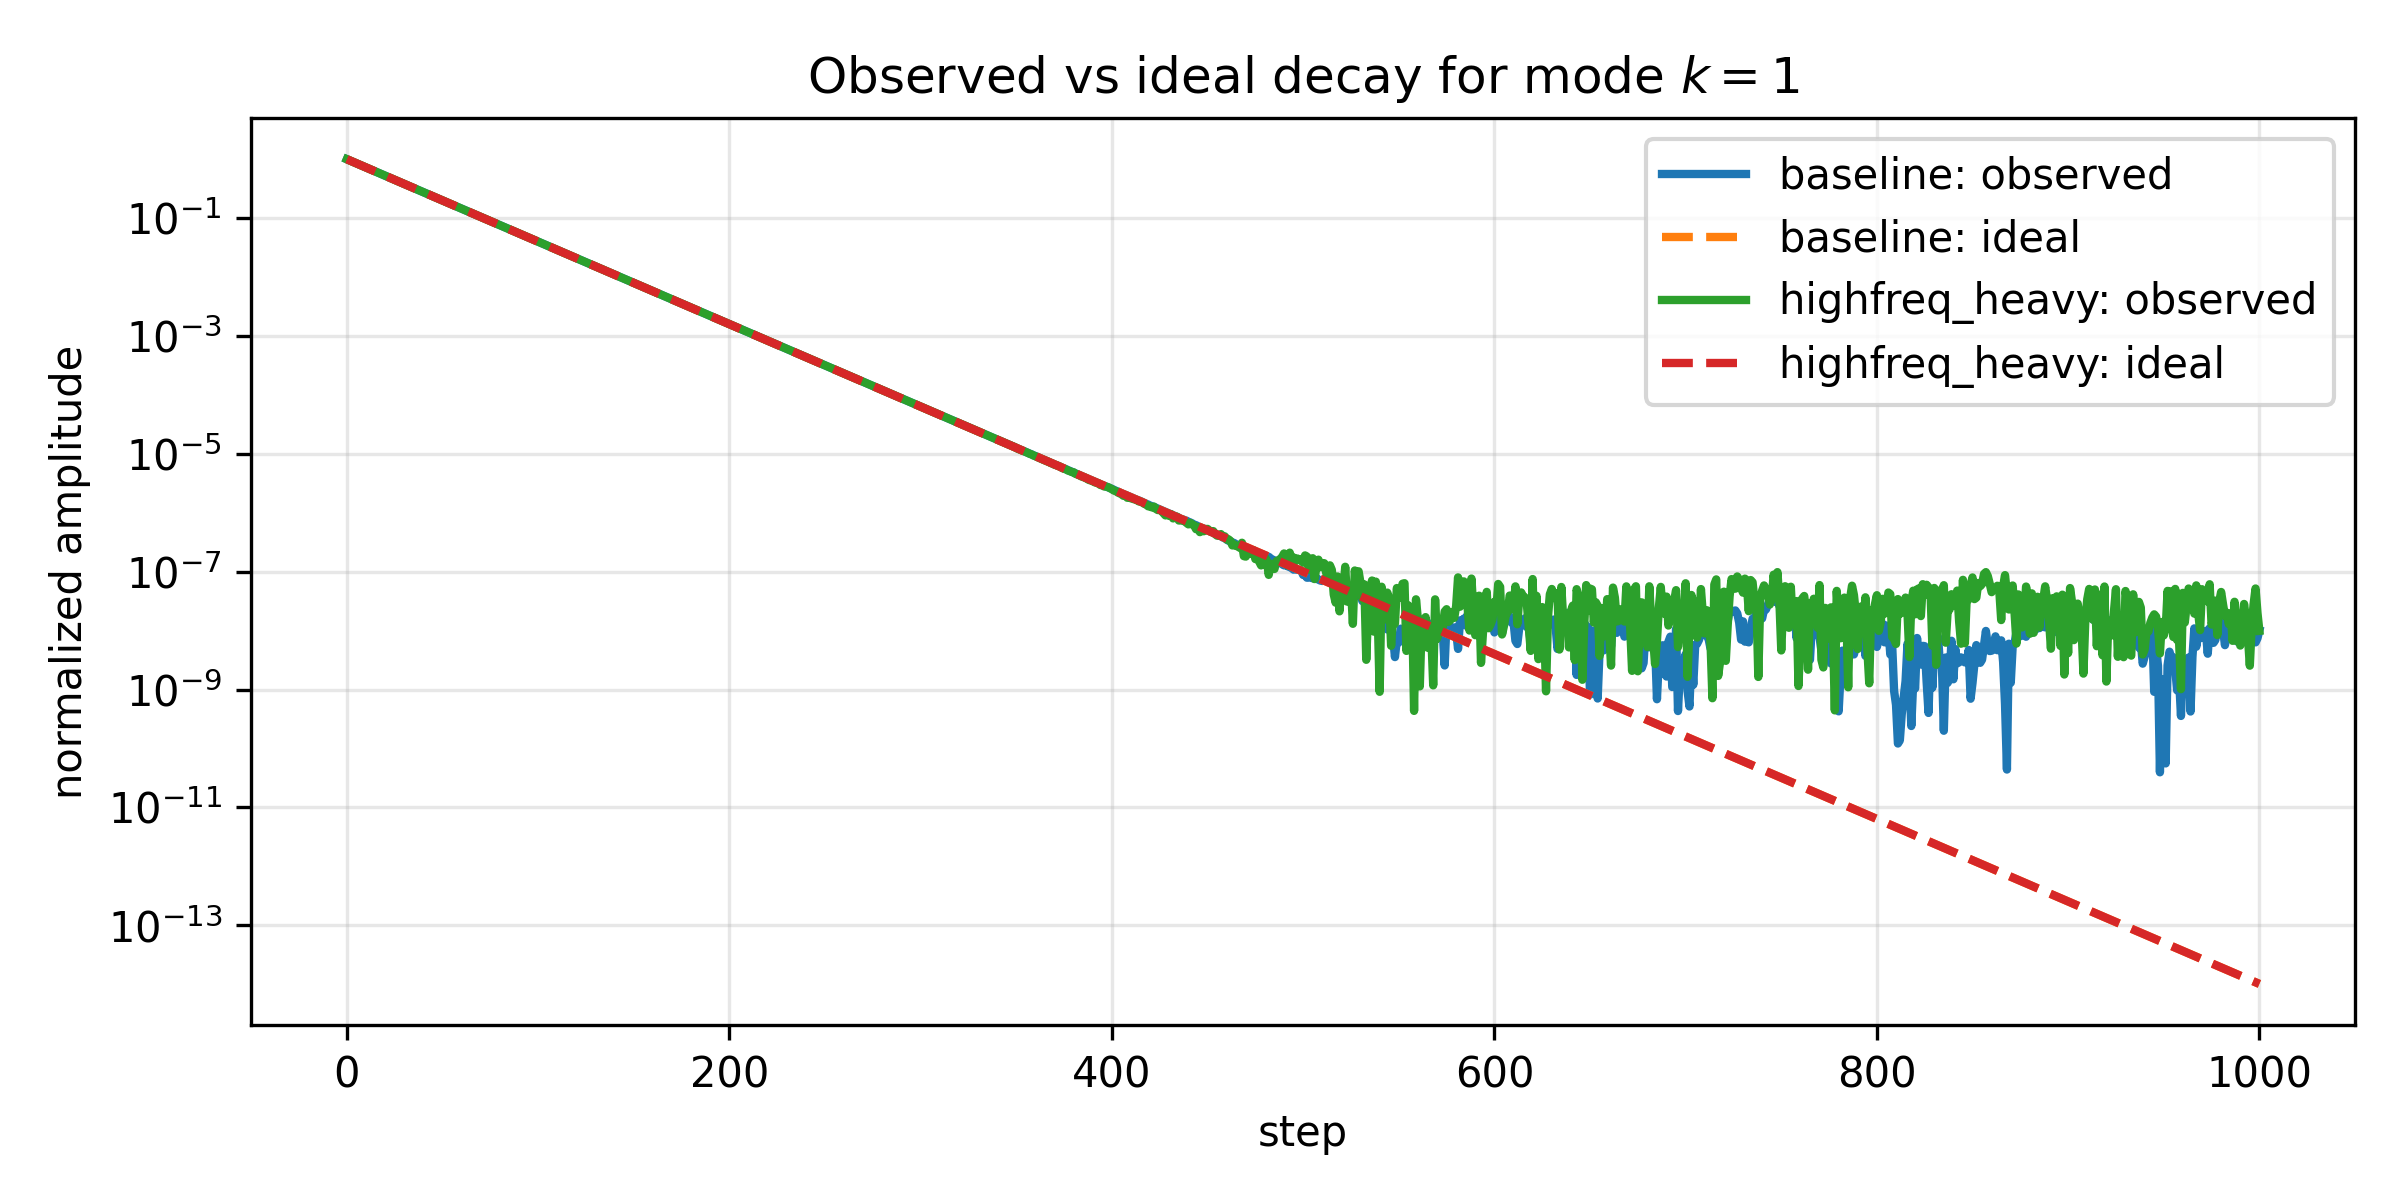
\includegraphics[width=\linewidth]{images/observed_vs_ideal_residual_decay_mode_1.png}
		\caption{Mode $k=1$}
	\end{subfigure}

	\vspace{0.6em}

	\begin{subfigure}[t]{0.48\textwidth}
		\centering
		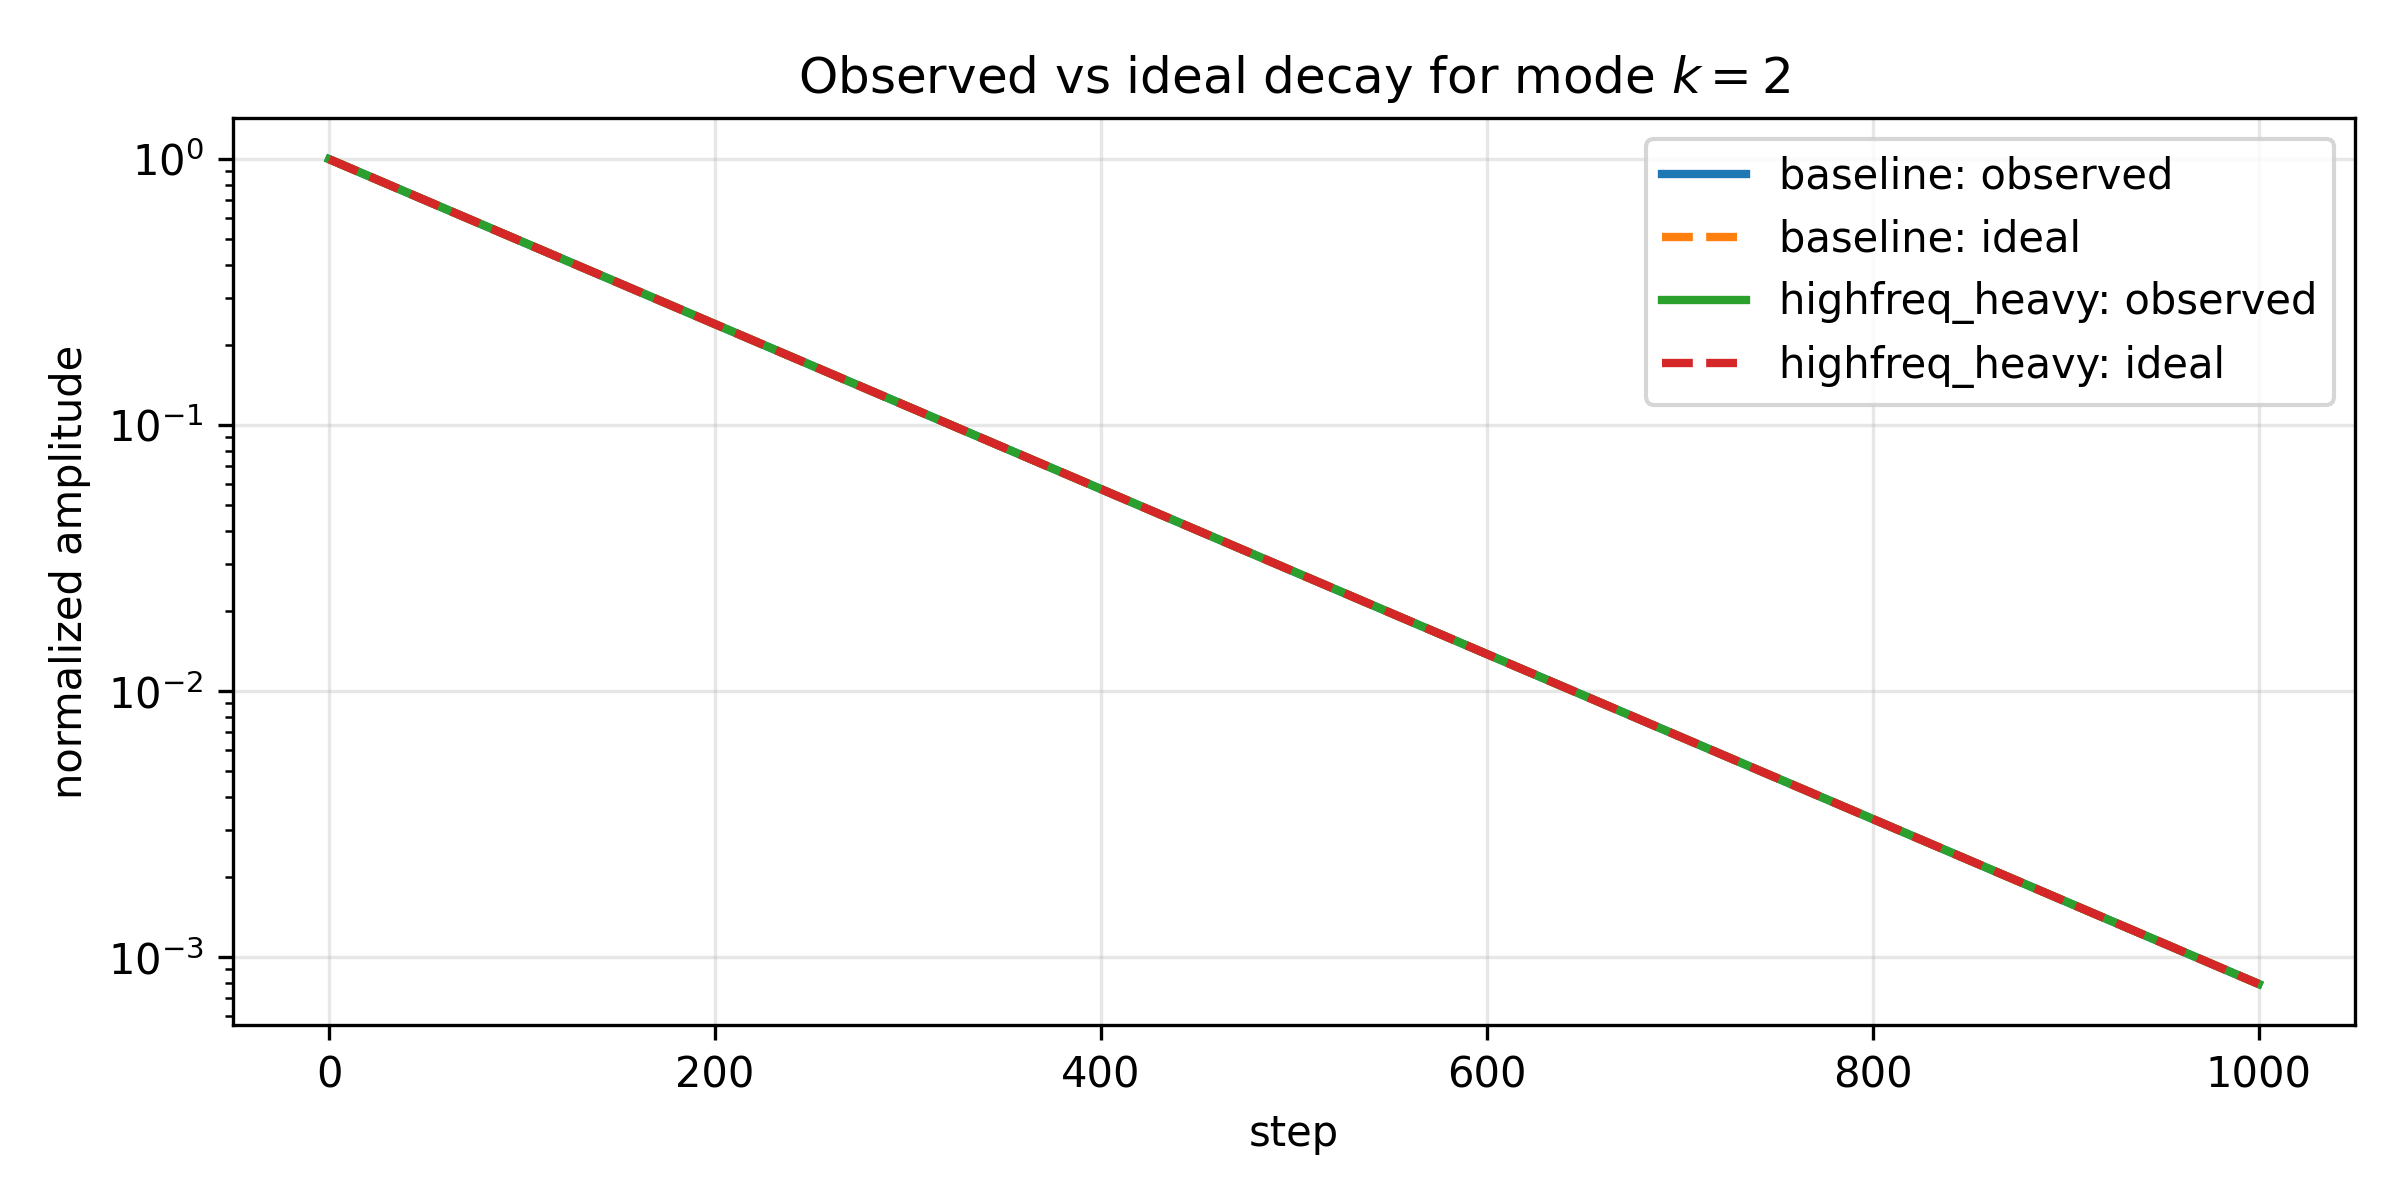
\includegraphics[width=\linewidth]{images/observed_vs_ideal_residual_decay_mode_2.png}
		\caption{Mode $k=2$}
	\end{subfigure}
	\hfill
	\begin{subfigure}[t]{0.48\textwidth}
		\centering
		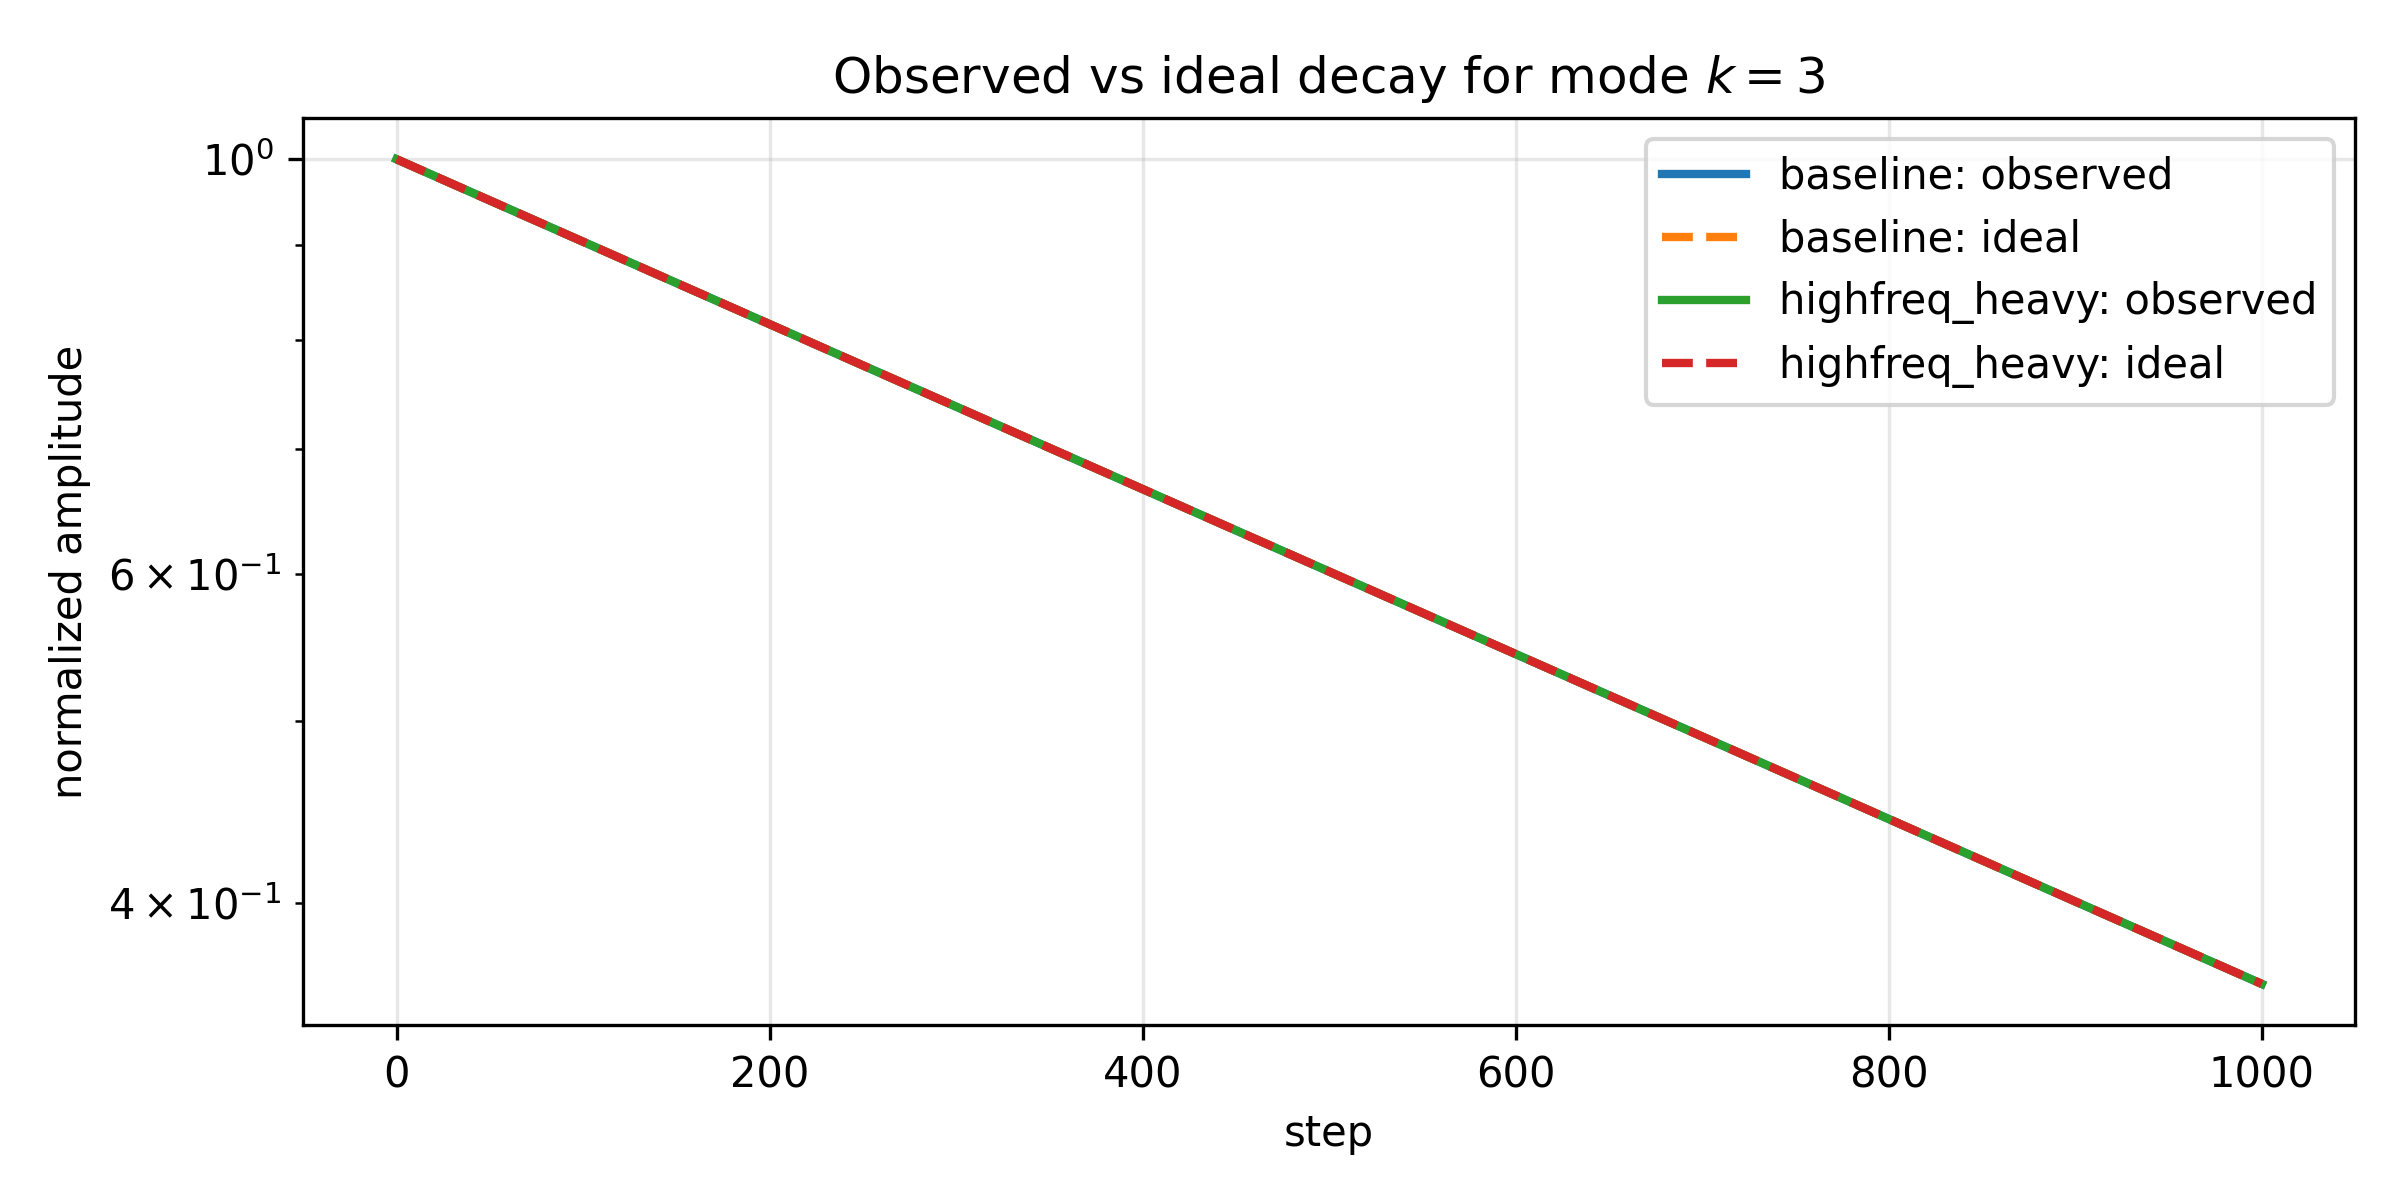
\includegraphics[width=\linewidth]{images/observed_vs_ideal_residual_decay_mode_3.png}
		\caption{Mode $k=3$}
	\end{subfigure}
	\caption{Observed versus ideal normalized residual decay for modes $k=0,1,2,3$.}
\end{figure}

\paragraph{Observations.}
\begin{itemize}
	\item For all four modes, the baseline and high-frequency-heavy runs follow the same normalized decay curves.
	\item This confirms the theoretical prediction
	      \[
		      r_k(t) = -\alpha_k(1-\eta\lambda_k^{\mathrm{emp}})^t,
	      \]
	      namely that $\alpha_k$ affects the initial scale, while $\lambda_k^{\mathrm{emp}}$ controls the decay rate.
	\item The ideal predictions are identical across the two experiments, and the observed curves lie on top of them up to numerical precision effects.
	\item For modes $k=0$ and $k=1$, both experiments hit the numerical floor after sufficient decay, so the curves flatten at machine precision.
	\item For modes $k=2$ and $k=3$, the observed and ideal curves remain essentially indistinguishable over the full time interval.
	\item Thus, increasing the amplitude of a higher-frequency component makes that component more prominent in the target, but does not make it converge faster.
\end{itemize}

\subsection*{Unnormalized mode decay}

\begin{figure}[H]
	\centering
	\begin{subfigure}[t]{0.48\textwidth}
		\centering
		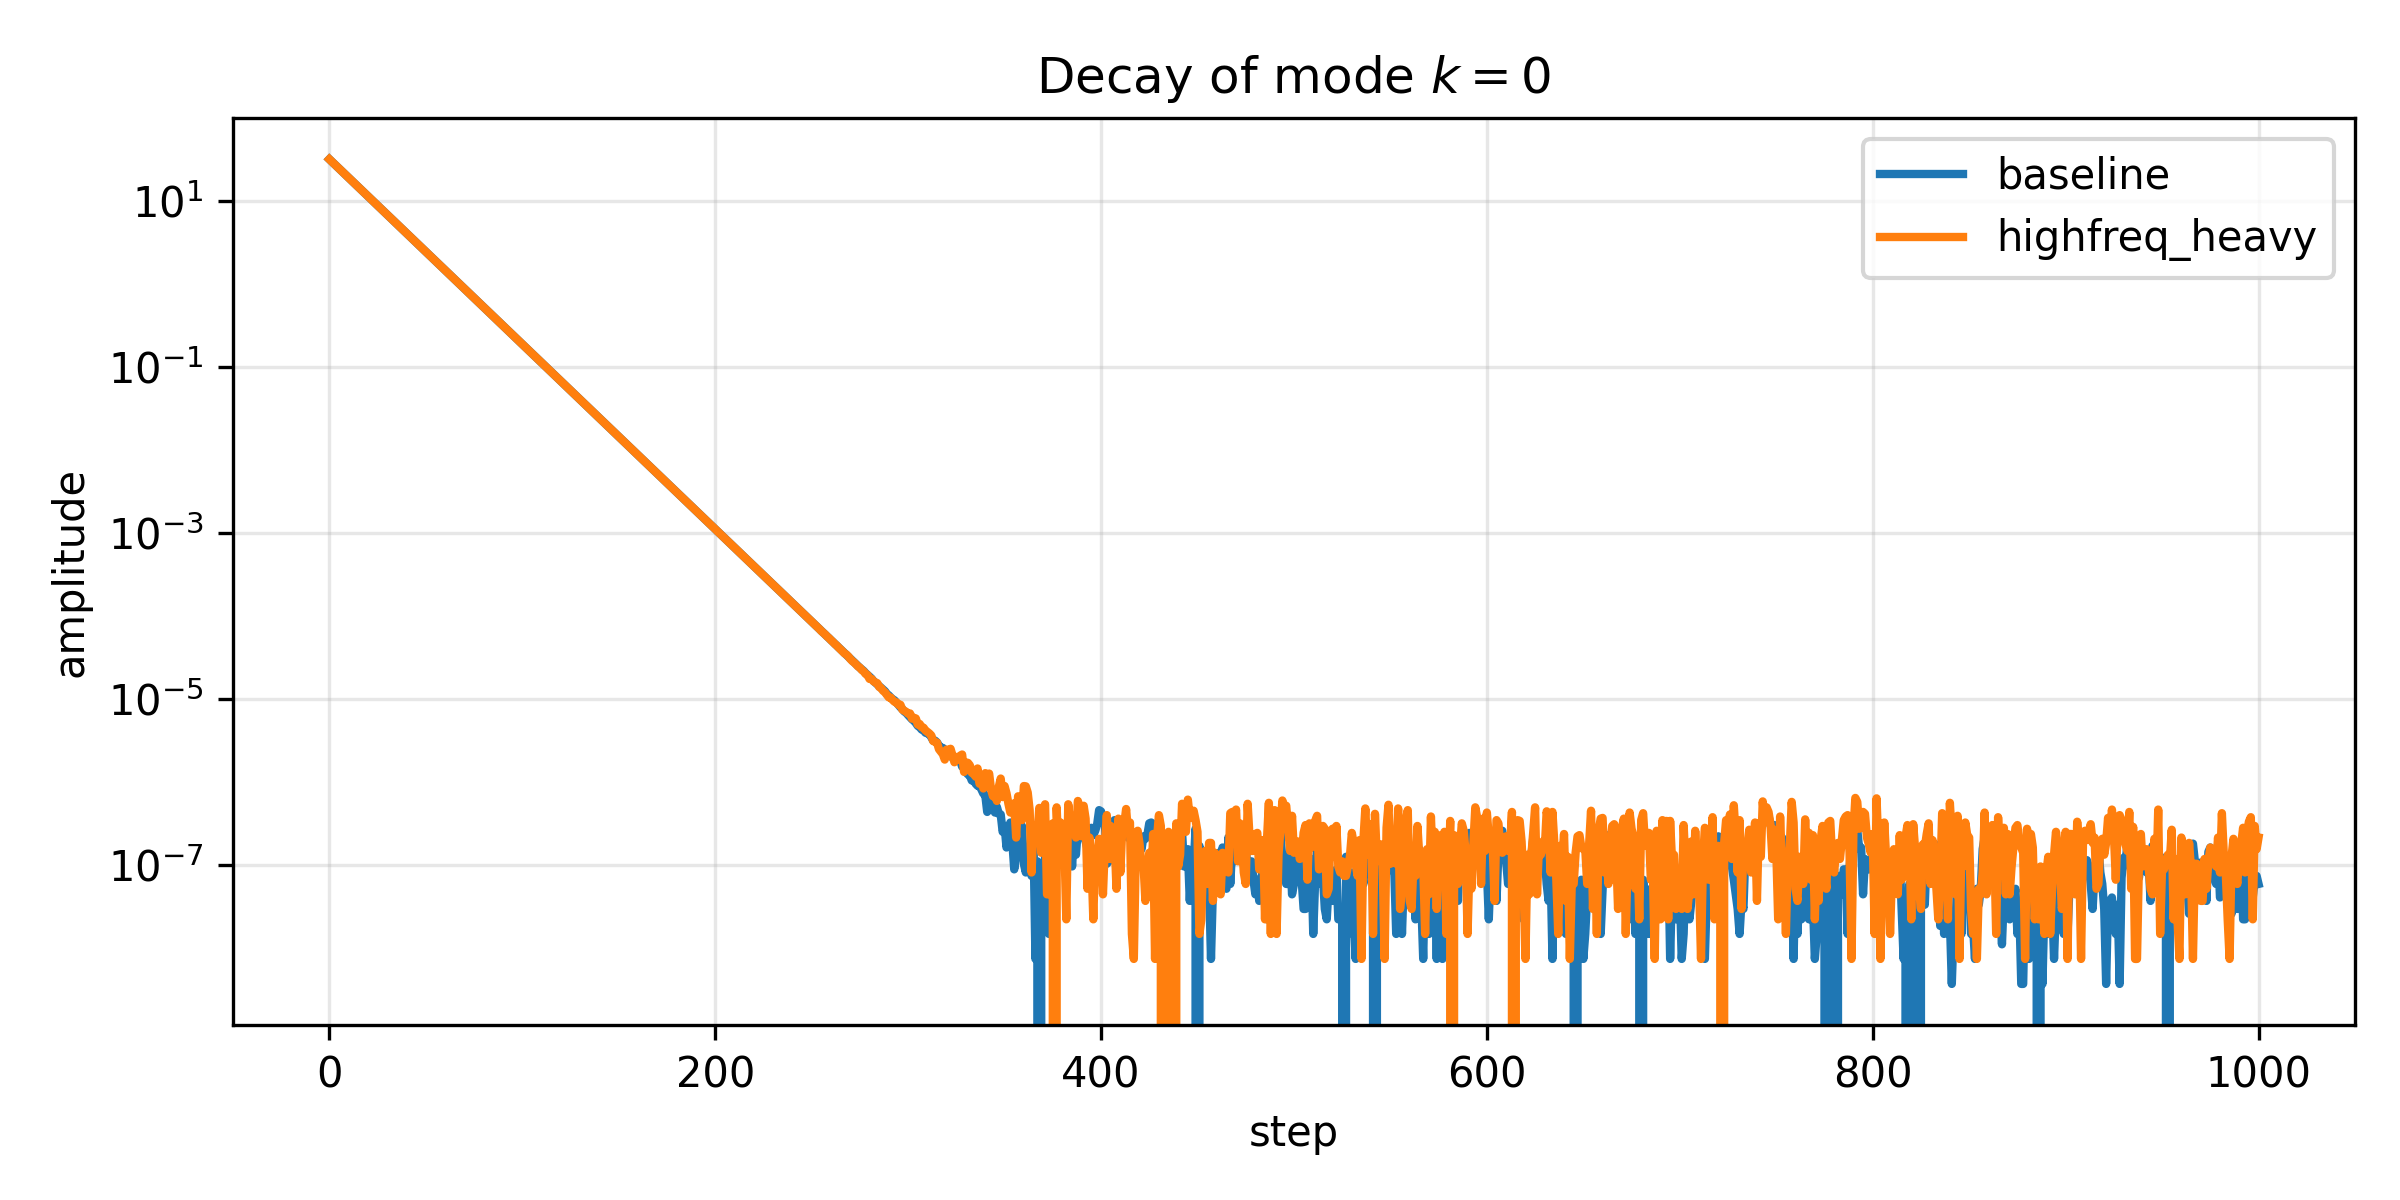
\includegraphics[width=\linewidth]{images/unnormalized_residual_decay_mode_0.png}
		\caption{Mode $k=0$}
	\end{subfigure}
	\hfill
	\begin{subfigure}[t]{0.48\textwidth}
		\centering
		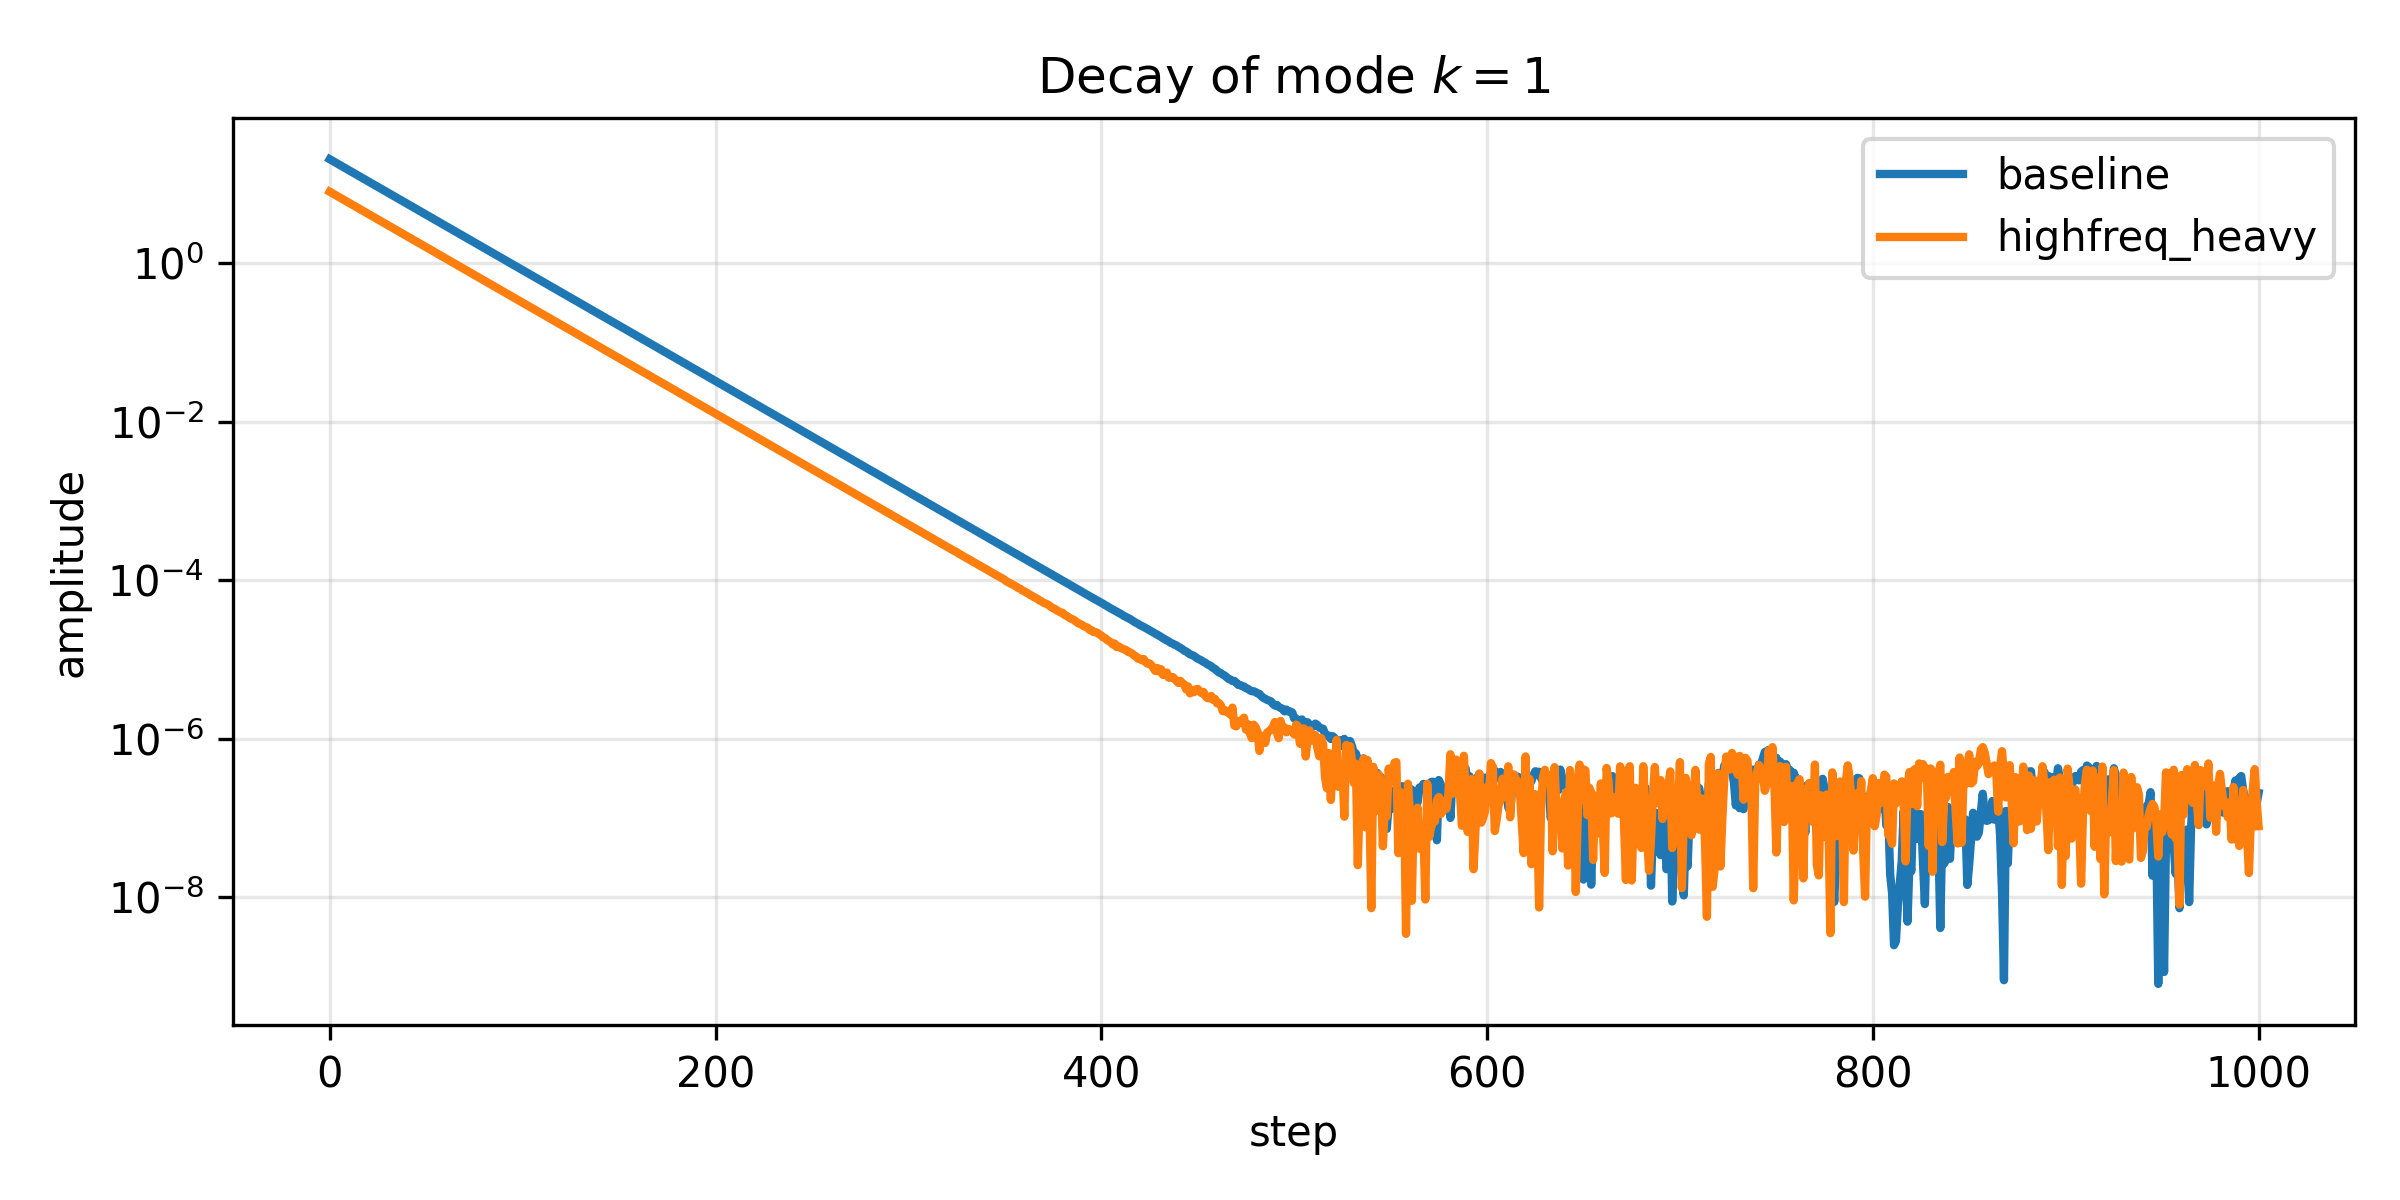
\includegraphics[width=\linewidth]{images/unnormalized_residual_decay_mode_1.png}
		\caption{Mode $k=1$}
	\end{subfigure}

	\vspace{0.6em}

	\begin{subfigure}[t]{0.48\textwidth}
		\centering
		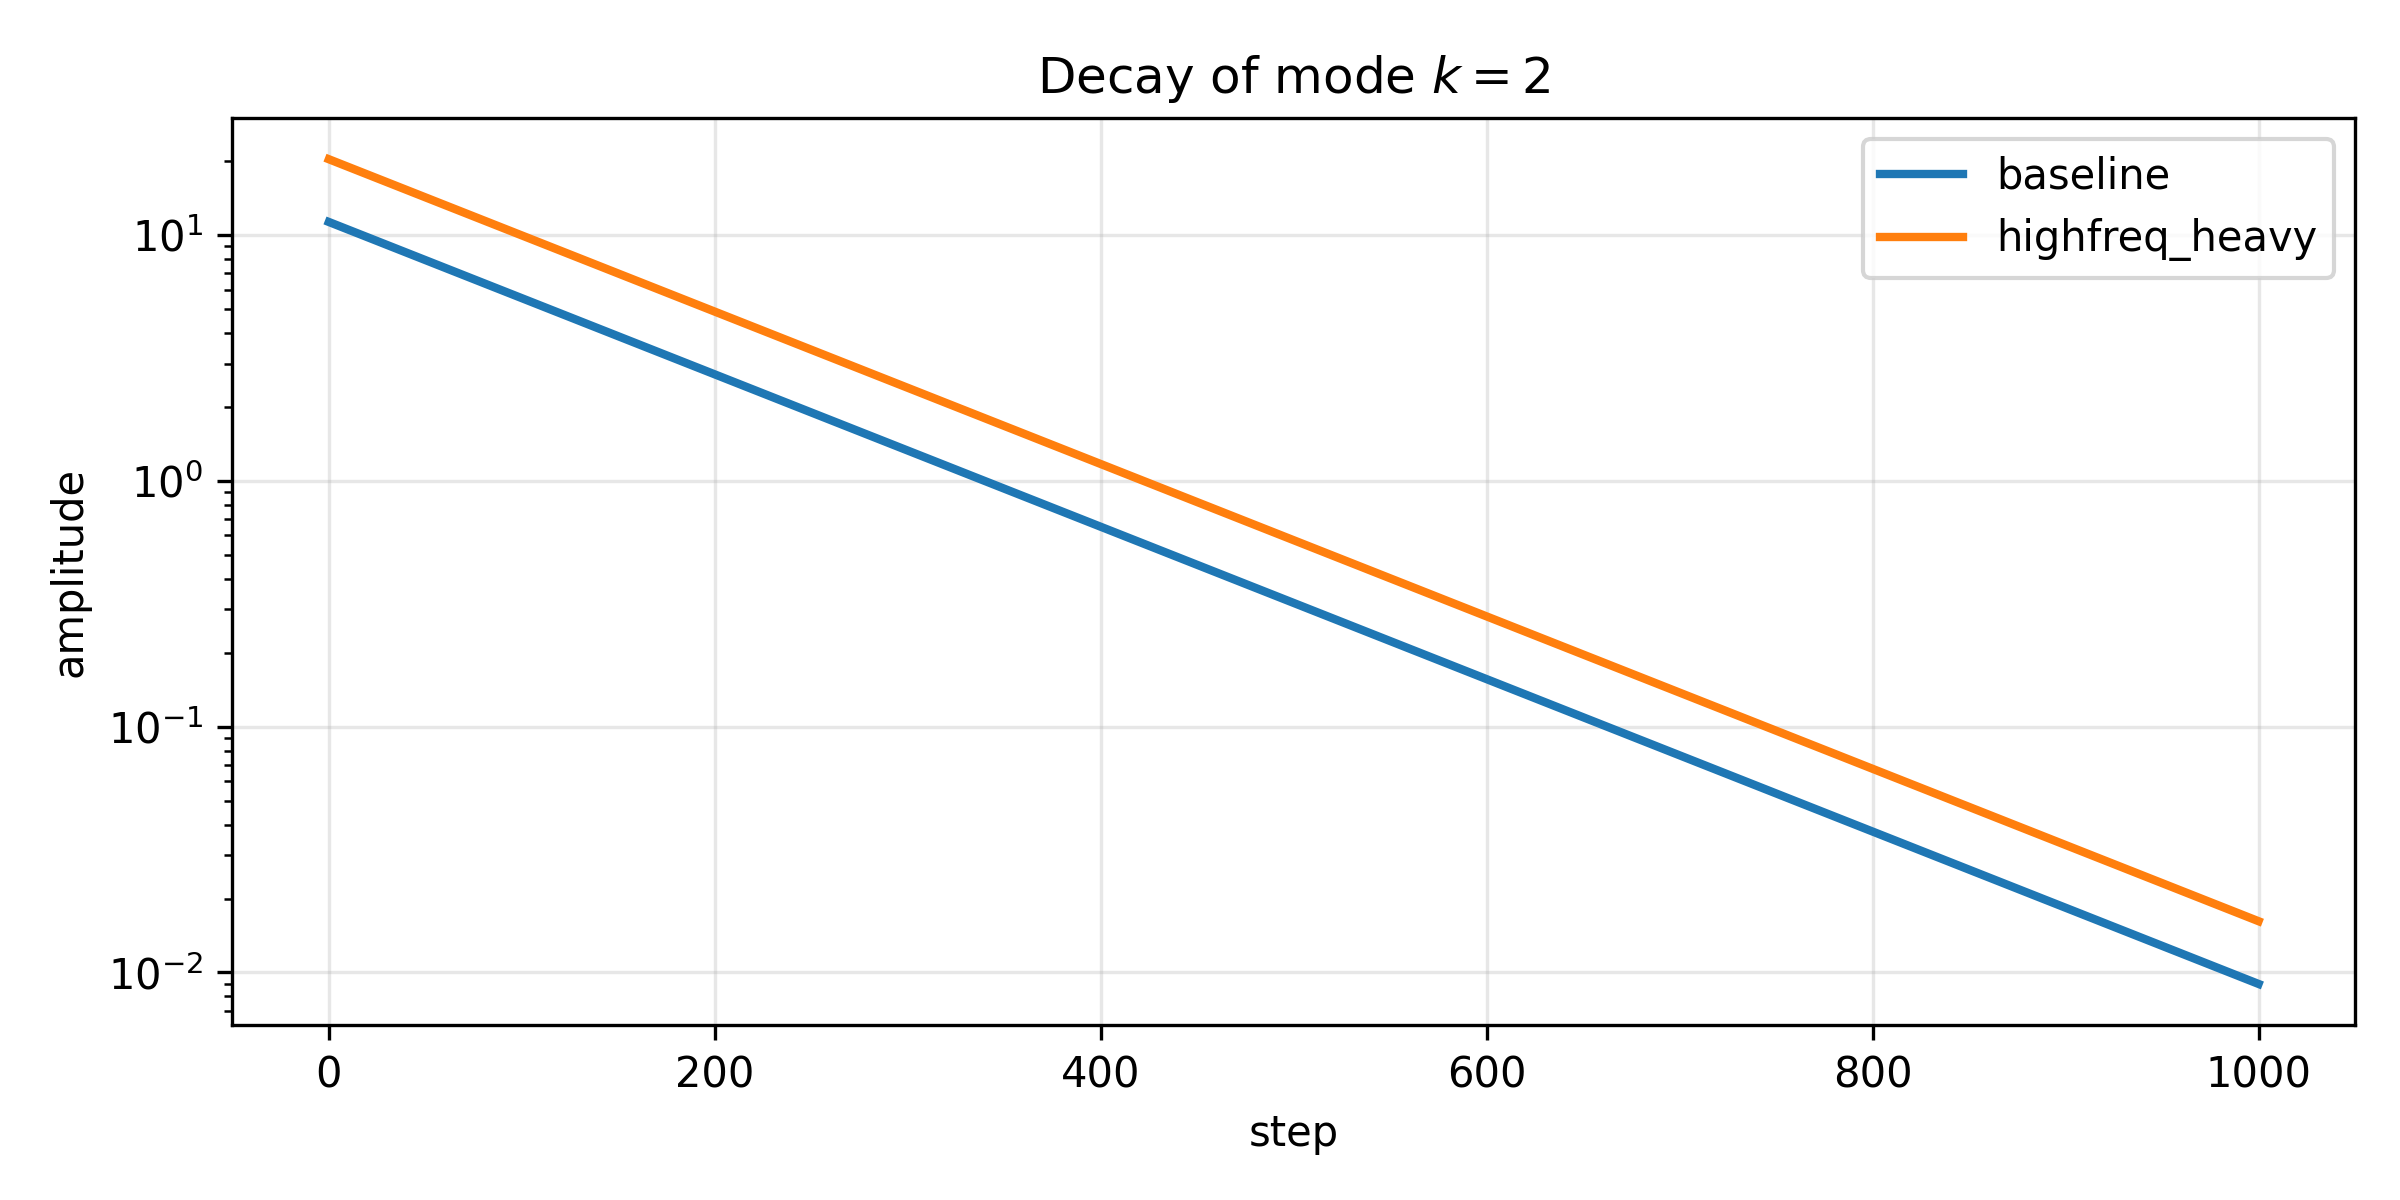
\includegraphics[width=\linewidth]{images/unnormalized_residual_decay_mode_2.png}
		\caption{Mode $k=2$}
	\end{subfigure}
	\hfill
	\begin{subfigure}[t]{0.48\textwidth}
		\centering
		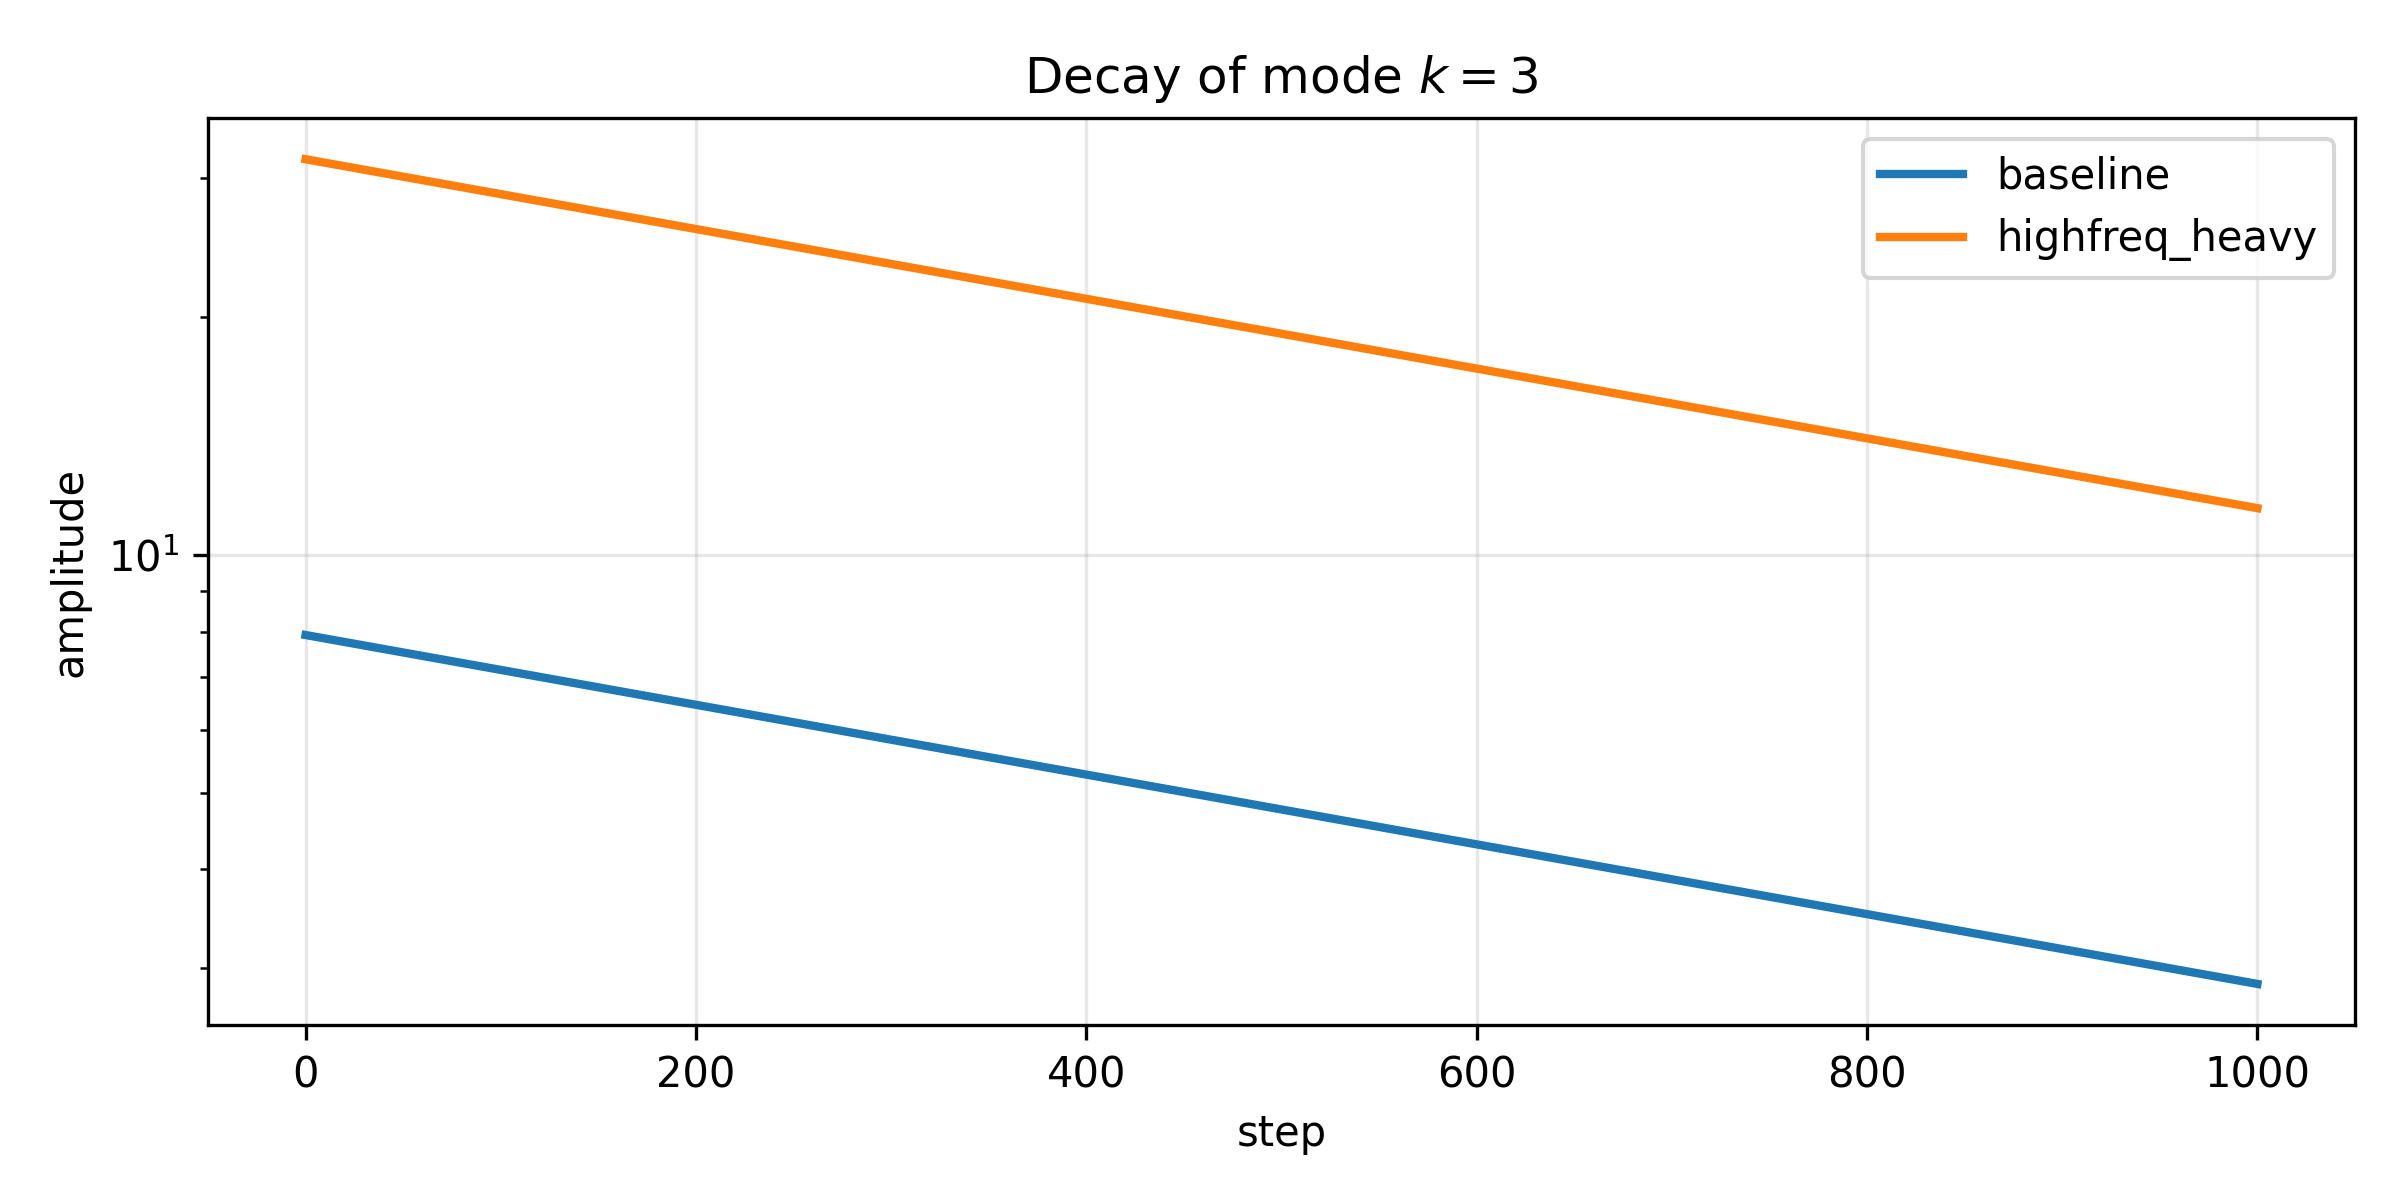
\includegraphics[width=\linewidth]{images/unnormalized_residual_decay_mode_3.png}
		\caption{Mode $k=3$}
	\end{subfigure}
	\caption{Observed unnormalized residual decay for the active modes.}
\end{figure}

\paragraph{Observations.}
\begin{itemize}
	\item The unnormalized mode amplitudes differ substantially between the baseline and high-frequency-heavy targets.
	\item In particular, the high-frequency-heavy experiment starts with much larger residual mass in the slower modes $k=2$ and $k=3$.
	\item Since these modes have smaller kernel eigenvalues, they decay more slowly in absolute magnitude and therefore dominate the residual for longer.
	\item This explains the overall loss gap: the high-frequency-heavy target is not converging more slowly because its per-mode rates changed, but because more of the initial target energy is concentrated in modes that are intrinsically slow.
\end{itemize}

\paragraph{Interpretation.}
For zero initialization,
\[
	r_k(t) = -\alpha_k (1-\eta\lambda_k^{\mathrm{emp}})^t.
\]
The normalized plots isolate the factor
\[
	(1-\eta\lambda_k^{\mathrm{emp}})^t,
\]
while the unnormalized plots retain the amplitude factor $\alpha_k$.
Hence:
\begin{itemize}
	\item normalized mode decay explains the \emph{rate},
	\item unnormalized mode decay explains the \emph{overall contribution to the loss}.
\end{itemize}

This is why the two experiments have nearly identical normalized decay curves but clearly different residual norms and final fitting quality.

\subsection*{Conclusion for the amplitude-swap experiment}

The baseline vs high-frequency-heavy comparison shows:
\begin{enumerate}
	\item Changing amplitudes changes the \emph{target shape} and the \emph{absolute fitting difficulty} at finite time.
	\item It does \emph{not} change the normalized mode-wise decay rates.
	\item The slower overall convergence in the high-frequency-heavy experiment is therefore explained by the fact that more energy is placed in the slower modes, not by a change in the kernel dynamics themselves.
\end{enumerate}

This is exactly the behavior predicted by standard kernel gradient descent on the equally spaced circle grid.
\end{document}
